
\chapter{遗忘理论在反应式系统中的应用}
\label{chapter04}
%{\em 本章针对第\ref{chapter01}章提出的问题(2)探讨使用遗忘的方法来解决计算反应式系统WSC(SNC)和知识更新。首先给出SNC (WSC)的定义,然后证明任意公式的SNC(WSC)可以规约到命题下的SNC(WSC)。并证明SNC和WSC是一对对偶概念,因此探讨其中一个就足以表示另一个的性质。其次,从遗忘的角度给出了计算SNC(WSC)的方法。基于此,当给定的反应式系统模型为有限状态时,可以事先将该模型用其特征公式表示出来,然后使用遗忘来计算其SNC(WSC)。
%	最后,提出使用遗忘定义
%	%反应式系统中$\CTL$和$\mu$-演算。。。。。。
%	知识更新的方法。

{\em
遗忘可以用于从本体中抽取摘要、隐蔽敏感信息、计算逻辑差等;
WSC和SNC在智能规划和形式化验证里有重要作用,例:在2003年,Lin使用WSC和SNC计算规划问题中的后继状态公理。
%在第\ref{chapter02}章中详细介绍了命题逻辑和模态逻辑S5下使用遗忘计算WSC(SNC)的方法和算法。
本章针对第\ref{chapter01}章提出的问题(2),研究$\CTL$和$\mu$-演算中如何使用遗忘计算反应式系统的SNC(WSC),及使用遗忘定义知识更新。即:
\begin{itemize}
	\item 对于给定的公式$\varphi$、原子命题$q$和原子命题集$V\subseteq \Var(\varphi)$,若满足$q \in \Var(\varphi)-V$,则$q$在$\varphi$和$V$上的SNC等价于公式$\varphi \wedge q$遗忘不在$V$中的原子命题后得到结果;WSC做为SNC的一个对偶概念,有相似的结论。而不终止的系统(包括反应式系统)在本章看作是一个有限的初始结构,本章将证明任意有限的初始结构(${\cal K}$)都能用其特征公式%(${\cal F}_{\Ha}({\cal K})$)
	来表示,因而可以使用遗忘的方法来计算其SNC(WSC)。
	\item 基于遗忘的知识更新通过极小改变现有知识的模型来使其适应新信息,这可以看作是基于模型的更新,且使用这种方法的更新满足katsuno等人提出的八条基本准则\cite{katsuno91mendelzon}。
\end{itemize}

本章其余部分组织如下:首先,第\ref{chapter06:sec:des}节给出有限初始结构的特征公式描述;其次,第\ref{chapter04:sec:snc}节给出最强必要条件和最弱充分条件的定义,探索这两个概念的相关性质,并给出基于遗忘的计算方法;然后,第\ref{chapter04:sec:update}节提出基于遗忘的知识更新方法,并证明其与基于偏序关系的方法等价;最后,总结本章的研究工作。}

\section{有限初始结构的特征公式}\label{chapter06:sec:des}%\label{sec:chapter06_chaIntC}
本小节介绍与一个初始结构相关的$\CTL$公式——特征公式。
为此,本节令初始结构为有限初始结构,即:原子命题集$\Ha$为有限集,且初始结构的状态为有限个。
%对于一个给定的有限初始结构(状态个数和$\Ha$都是有限的),其不循环的计算树(状态不重复出现)的深度最多为其状态数的个数。
对于一个给定的初始结构,其特征公式与其计算树的特征公式密切相关。
因此,本小节首先介绍计算树之间的$V$-互模拟关系;然后,给出计算树的特征公式的定义;最后,给出初始结构的特征公式。

\subsection{计算树$V$-互模拟}
第\ref{chapter03}章中的定义\ref{def:VInd:bisimulation}给出了$\Ind$- 结构之间的$V$-互模拟定义及其相关性质,结构之间的$V$-互模拟有相同的定义,即:$\Ind$-结构之间$V$-互模拟具有的性质都可以平凡的迁移到结构之间$V$-互模拟。
这里给出有限结构间有界$V$-互模拟(与深度$n$关联的$V$-互模拟)的定义,并证明$V$-互模拟与有界$V$-互模拟在有限结构下等价。
%本节给出结构之间的$V$-互模拟在有限结构下与下面将要给出的有界$V$-互模拟——与深度$n$关联的$V$-互模拟等价。
%但是为了方便,本章仍然引入有界$V$-互模拟的概念。
因此,第\ref{chapter03}章遗忘有的性质在本章约束情形下基本也有~\cite{renyansfirstpaper},这里不再赘述。

首先给出能够描述一定深度$n\in \mathbb{N}$的计算树之间的$V$-互模拟关系,记为$\Hb_n^V$。令$V\subseteq \Ha$是原子命题集,$i\in \{1,2\}$,$\Hm_i=(S_i,R_i,L_i,s_0^i)$是初始Kripke结构,${\cal K}_i=(\Hm_i, s_i)$是结构。$\Hb_n^V$递归定义如下:
\begin{itemize}
	\item 若$L_1(s_1)-V=L_2(s_2)$,则$({\cal K}_1,{\cal K}_2) \in \Hb_0^V$;
	\item 对任意$n\ge 0$,若满足下面几个条件,则$({\cal K}_1,{\cal K}_2)\in \Hb_{n+1}^V$成立:
	\begin{itemize}
		\item $({\cal K}_1,{\cal K}_2) \in \Hb_0^V$;
		\item 对任意$(s_1,s_1')\in R_1$,存在$(s_2,s_2')\in R_2$,使得$({\cal K}_1',{\cal K}_2') \in \Hb_n^V$;
		\item 对任意$(s_2,s_2')\in R_2$,存在$(s_1,s_1')\in R_1$,使得$({\cal K}_1',{\cal K}_2') \in \Hb_n^V$。
	\end{itemize}
\end{itemize}
其中${\cal K}_i'=(\Hm_i,s_i')$。

当所谈及的原子命题集$V$很显然的时候,上述$\Hb_n^V$中的$V$可以省略,记为$\Hb_n$。此外,当讨论的$\Hm_i$ $(i=1,2)$是显然的时候,可以使用$(s_1,s_2) \in \Hb_n$代替$((\Hm_1,s_1),(\Hm_2,s_2))$ $\in \Hb_n$。
有界$V$-互模拟关系就可以定义如下:
\begin{definition}[有界$V$-互模拟]\label{def:V-bisimulation}
	令$V$是$\Ha$的一个子集,$i\in \{1,2\}$, ${\cal K}_1$和${\cal K}_2$是结构。
	\begin{itemize}
		\item ${\cal K}_1$和${\cal K}_2$是有界$V$-互模拟的,当且仅当对所有$n \ge 0$,都有$({\cal K}_1, {\cal K}_2)\in \Hb_n$。若 ${\cal K}_1$ 和 ${\cal K}_2$是有界$V$-互模拟的,则记为${\cal K}_1 \overset{B}{\lrto}_V {\cal K}_2$。
		\item 对$\Hm_i$上的路径$\pi_i=(s_{i,1},s_{i,2},\dots)$,若对于任意$j\in \mathbb{N}_{\ge 1}$\footnote{$\mathbb{N}$为整数集,$\mathbb{N}_{\ge 1}$是大于等于1的整数集。},都有${\cal K}_{1,j} \overset{B}{\lrto}_V {\cal K}_{2,j}$,则$\pi_1 \overset{B}{\lrto}_V \pi_2$。其中${\cal K}_{i, j}=(\Hm_i, s_{i,j})$。
	\end{itemize}
\end{definition}

值得注意的是,满足有界$V$-互模拟关系的结构之间有且仅有一个有界$V$-互模拟关系,即$\Hb_{k+1} = \Hb_k$($k \in \mathbb{N}$)。
%上述约束$V$-互模拟的定义是现有互模拟定义的一般化,这可以从下面几个方面来体现\footnote{在其他领域也有类似的定义,如:定义在数据库相关文献中的概念$k$-互模拟\cite{kaushik2002updates}。$k$-互模拟概念中涉及与本文$\Hb_n$类似的定义,只是其关系是从相反的方向(即:从孩子到父节点的方向)来说明的。此外,值得一提的是,本文的$V$-互模拟的概念是定义在$\MPK$-结构上的。}。
%首先,当给定的$V$为空集且谈论指定的初始状态时,本文的$V$-互模拟与定义在Baier 等文章里的互模拟等价(定义7.1\cite{Baier:PMC:2008})的概念一致。
%其次,在上述文章里的基于状态的互模拟(定义7.7\cite{Baier:PMC:2008})是定义在给定结构的状态上的,因此与本文的$V$- 互模拟(定义在结构的集合上)也不同。
%最后,本文的$\Hb_n$的定义与Browne的论文中的状态等价$E_n$类似,只是后者是定义在状态上\cite{browne1988characterizing} 而本文的定义在$\MPK$-结构(或$\Ind$-结构)上。


\begin{lemma} \label{lem:HbBis}
	对于有限初始Kripke结构,有界 $V$-互模拟是一个 $V$-互模拟。
	%Let $V \subseteq \Ha$ and ${\cal K}_i=({\cal M}_i,s_i)~(i\in\{1,2\})$ and $\Hm_i=(S_i, R_i,L_i, s_0^i)$ be finite initial structures.
	%Then every bounded $V$-bisimulation is a $V$-bisimulation between $\Hm_1$ and $\Hm_2$.
	%If $s_1 \lrto_V s_2$, then the bounded $V$-bisimulation {\cal B}_V containing $(s_1, s_2)$ is also a $V$-bisimulation (containing $(s_1,s_2)$) between $\Hm_1$ and $\Hm_2$.
\end{lemma}

\begin{proof}
	令 $V \subseteq \Ha$、 ${\cal K}_i=({\cal M}_i,s_i)~(i\in\{1,2\})$且$\Hm_i=(S_i, R_i,L_i, s_0^i)$为有限的初始-Kripke结构。
	因为$S_i~(i=1,2)$是有限的,所以$\Hb_n\subseteq S_1\times S_2~(n\ge 0)$ 都是有限的。
	由于对任意$n\geq 0$,都有 $\Hb_{n+1} \subseteq \Hb_n$。
	因此,存在一个最小数$k$,使得
	$\Hb_{k+1} =\Hb_k$(用 $\Hb$表示)。
	
	
	下证对任意 $r_1\in S_1$和 $r_2 \in S_2$,若$(r_1, r_2)\in \Hb$,则 %if and only if
	\begin{itemize}
		\item[(a)] $L_1(r_1)-V = L_2(r_2)-V$;
		\item[(b)] $\forall w_1\in S_1$,若$(r_1, w_1)\in R_1$,则 $\exists w_2 \in S_2$,使得 $(r_2,w_2) \in R_2$和 $(w_1, w_2) \in \Hb$;
		\item[(c)] $\forall w_2\in S_2$,若$(r_2, w_2)\in R_2$,则 $\exists w_1 \in S_1$,使得 $(r_1,w_1) \in R_1$和 $(w_1, w_2)\in \Hb $。
	\end{itemize}
	
	首先,由对任意$n\ge 0$,都有$(r_1, r_2)\in \Hb_n$,可知$(r_1, r_2) \in \Hb_0$,这表明
	$L_1(r_1)-V = L_2(r_2)-V$。因此(a) 成立。
	
	其次,令$w_1 \in S_1$和 $(r_1, w_1)\in R_1$。有 \\
	$(r_1,r_2)\in \Hb$、 $w_1 \in S_1$ 和 $(r_1, w_1)\in R_1$\\
	$\Rto$ 由$\Hb_{k+1}=\Hb$可知$(r_1,r_2)\in \Hb_{k+1}$、 $w_1 \in S_1$和 $(r_1, w_1)\in R_1$\\
	$\Rto$ 由定义可知$\exists w_2\in S_2$,使得 $(r_2, w_2)\in R_2$和 $(w_1,w_2)\in \Hb_k$\\
	$\Rto$ 由$\Hb=\Hb_k$可知$\exists w_2\in S_2$,使得 $(r_2, w_2)\in R_2$和 $(w_1,w_2)\in \Hb$\\
	$\Rto$ (b)成立。
	
	可以类似地证明 (c)也成立。
	因此, $\Hb$是$\Hm_1$和 $\Hm_2$之间的一个 $V$-互模拟关系。
\end{proof}

由引理\ref{lem:HbBis}可知,$\Hb$既是一个有界$V$-互模拟关系也是一个$V$-互模拟关系。因此,下面的推论显然成立。
\begin{corollary} \label{lem:bounedToGe}
	令 $V \subseteq \Ha$ 和 ${\cal K}_i=({\cal M}_i,s_i)$( $i\in\{1,2\}$)。若$\Hm_i=(S_i, R_i,L_i, s_0^i)$是有限的初始Kripke 结构,则
	%$s_1 \overset{\Hb}{\lrto}_V s_2$
	$s_1$和 $s_2$是有界 $V$-互模拟的,当且仅当$s_1 \lrto_V s_2$。
\end{corollary}


本章只涉及有限的初始Kripke结构,因此,本章用$\lrto_V$($V$-互模拟)表示$\overset{B}{\lrto}_V $(有界$V$-互模拟)。

给定原子命题集$V\subseteq \Ha$和初始Kripke结构$\Hm_i$($i = 1, 2$)。如果下面条件同时满足:
\begin{itemize}
	\item $L_1(s_1)- V=L_2(s_2)- V$,
	%   \item For every subtree $\Tr_{n-1}(s_i')$ of $\Tr_n(s_i)$,
	%   $\Tr_n(s_{(i \mod 2)+1})$ has a subtree $\Tr_{n-1}(s_{(i \mod 2)+1}')$ such that
	%   $\Tr_{n-1}(s_i')\lrto_V\Tr_{n-1}(s_{(i \mod 2)+1}')$.
	\item 对$\Tr_n(s_1)$的任意子树$\Tr_{n-1}(s_1')$,都存在  $\Tr_n(s_2)$的子树$\Tr_{n-1}(s_2')$,使得
	$\Tr_{n-1}(s_1')\lrto_V\Tr_{n-1}(s_2')$,且
	\item 对任意$\Tr_n(s_2)$的子树$\Tr_{n-1}(s_2')$,都存在$\Tr_n(s_1)$ 的子树$\Tr_{n-1}(s_1')$,使得
	$\Tr_{n-1}(s_1')\lrto_V\Tr_{n-1}(s_2')$;
\end{itemize}
则称$\Hm_1$的计算树$\Tr_n(s_1)$和$\Hm_2$的计算树$\Tr_n(s_2)$是$V$-互模拟的(记为$({\cal M}_1,\Tr_n(s_1))\lrto_V({\cal M}_2,\Tr_n(s_2))$,简写为$\Tr_n(s_1)\lrto_V\Tr_n(s_2)$)。

特别地,当$n=0$时,只需考虑第一个条件即可。

\begin{proposition}\label{B_to_T}
	给定原子命题集$V\subseteq\cal A$和结构$({\cal M}_i,s_i)$($i=1,2$)。
	那么:
	\[(s_1,s_2)\in{\cal B}_n\mbox{当且仅当对任意$0\le j\le n$,有}
	\Tr_j(s_1)\lrto_V\Tr_j(s_2)\mbox{。}\]
\end{proposition}
\begin{proof}
	下面从两个方面来证明这一结论。
	
	$(\Rto)$ 下证“如果$(s_1, s_2) \in \Hb_n$,则对于任意$0 \leq j \leq n$,有$Tr_j(s_1) \lrto_V Tr_j(s_2)$”成立。$(s_1, s_2) \in \Hb_n$表明$Tr_n(s_1)$和$Tr_n(s_2)$的根有同样的标签(除了$V$里的元素之外)。
	此外,对任意$(s_1, s_{1,1}) \in R_1$,存在一个$(s_2, s_{2,1})\in R_2$,使得$(s_{1,1}, s_{2,1}) \in \Hb_{n-1}$;且对任意$(s_2, s_{2,1})\in R_2$,存在一个$(s_1, s_{1,1}) \in R_1$,使得$(s_{1,1}, s_{2,1}) \in \Hb_{n-1}$。
	因此,由定义可知$Tr_1(s_1)$ $\lrto_V Tr_1(s_2)$。递归地使用上述方法可得对任意$0 \leq j \leq n$,都有$Tr_j(s_1) \lrto_V Tr_j(s_2)$。
	
	$(\Lto)$下证“如果对于任意$0 \leq j \leq n$有$Tr_j(s_1) \lrto_V Tr_j(s_2)$,则$Tr_j(s_1) \lrto_V Tr_j(s_2)$”成立。
	由$Tr_0(s_1) \lrto_V Tr_0(s_2)$可知$L(s_1) - V = L'(s_2) - V$,因而$(s_1, s_2) \in \Hb_0$。
	由$Tr_1(s_1) \lrto_V Tr_1(s_2)$可知$L(s_1) - V = L'(s_2)- V$,且对于一棵树根的任意后继状态$s$,都能找到另一棵树根的一个后继状态$s'$,使得$(s, s')\in \Hb_0$。
	因此,$(s_1, s_2) \in \Hb_1$。同理可证$(s_1, s_2) \in \Hb_2$, \dots, $(s_1, s_2) \in \Hb_n$。
\end{proof}

命题\ref{B_to_T}表明,任意两个初始结构中的两个状态$s_1$和$s_2$能够在$\overline{V}$上相互模拟对方直到$n$步,当且仅当分别以$s_1$和$s_2$为根的计算树能在$\overline{V}$上相互模拟直到深度为$n$。
由此可知,如果同一初始结构的两个状态$s$ 和$s'$不是$V$-互模拟的,则存在一个数$k\in \mathbb{N}$,使得分别以$s$和$s'$ 为根的计算树$\Tr_k(s)$和$\Tr_k(s')$不是$V$-互模拟的。
\begin{proposition}\label{pro:k}
	给定原子命题集$V\subseteq \Ha$、初始Kripke结构$\Hm$和两个状态$s,s'\in S$。
	若$s\not\lrto_V s'$,则存在一个最小整数$k$,使得$\Tr_k(s)$和$\Tr_k(s')$不是$V$-互模拟的。
\end{proposition}
\begin{proof}
	若$s\not\lrto_V s'$,则存在一个最小的数$c$,使得$(s_i, s_j) \notin \Hb_c$。因此,由命题\ref{B_to_T}可知,存在一个最小整数$m$($m \leq c$),使得$\Tr_m(s_i)$和 $\Tr_m(s_j)$不是$V$-互模拟的。令$k=m$可得上述结论。
\end{proof}


\subsection{计算树的特征公式}
由上面小节的讨论可知,$V$-互模拟可以将计算树区别开\footnote{相似的方法在Mycielski等人的文章中已被使用~\cite{DBLP:conf/birthday/1997ehrenfeucht},在这篇文章中一元公式的结构通过等价类$\equiv_{\overline{k}}$被描述为Hintikka 公式~\cite{hintikka1953distributive}。 另一个类似的工作是Yankov-Fine构造~\cite{yankov1968three}。}。下面讨论如何使用$\CTL$公式描述计算树,且表明具有(或没有)$V$-互模拟关系的计算树的特征公式之间的关系。为此,首先给出计算树特征公式的定义。
\begin{definition}\label{def:V:char:formula}
	给定原子命题集$V\subseteq \Ha$、初始Kripke结构$\Hm =(S,R,L,s_0)$和状态$s\in S$。
	定义在$V$上的计算树$\Tr_n(s)$的特征公式(记为${\cal F}_V(\Tr_n(s))$,$n\geq 0$)递归定义如下:
	\begin{align*}
		{\cal F}_V(\Tr_0(s)) &=  \bigwedge_{p \in V\cap L(s)}p
		\wedge \bigwedge_{q\in V-L(s)} \neg q,\\
		{\cal F}_V(\Tr_{k+1}(s))& = \bigwedge_{(s,s')\in R}
		\EXIST \NEXT {\cal F}_V(\Tr_k(s'))
		\wedge
		\ALL \NEXT \bigg( \bigvee_{(s,s')\in R} {\cal F}_V(\Tr_k(s')) \bigg) \wedge {\cal F}_V(\Tr_0(s)) \hbox{ ($k\ge 0$)。}
	\end{align*}
\end{definition}

由定义\ref{def:V:char:formula}可知,计算树的特征公式从三个方面展示了计算树的信息:
\begin{itemize}
	\item[(1)] 只考虑$V$中的原子命题;
	\item[(2)] 突出了树节点的内容,即:对于任意原子命题$p\in V$,若$p$在节点的标签中,则其正出现在特征公式中,否则负出现在特征公式中;
	\item[(3)] 公式中的时序算子表示了状态之间的转换关系。
\end{itemize}
通俗一点,${\cal F}_V(\Tr_0(s))$表明了节点$s$的在$V$上的内容;$\EXIST \NEXT$ 的合取部分和$\ALL \NEXT$部分保证,以$s$ 的每个直接后继状态$s'$为根、深度为$k$的计算树都有一个$\CTL$公式来描述。

下面的结论表明,若两个计算树是$V$-互模拟的,则它们在$V$上的特征公式是逻辑等价的。
\begin{lemma}\label{lem:Vb:TrFormula:Equ}
	给定原子命题集$V\subseteq \Ha$、初始Kripke结构$\Hm=(S,R,L,s_0)$和$\Hm'=(S',R',L',s_0')$、$s\in S$、$s'\in S'$且 $n\ge 0$。若$\Tr_n(s) \lrto_{\overline V} \Tr_n(s')$,则${\cal F}_V(\Tr_n(s)) \equiv {\cal F}_V(\Tr_n(s'))$。
\end{lemma}
\begin{proof}
	通过归纳计算树的深度$n$来证明。
	
	\textbf{基始($n=0$):} 对任意$s_x\in S$和$s_x' \in S'$,若$\Tr_0(s_x) \lrto_{\overline V} \Tr_0(s_x')$,则由$L(s_x) - \overline V = L'(s_x') - \overline V$可知${\cal F}_V(\Tr_0(s_x)) \equiv {\cal F}_V(\Tr_0(s_x'))$。
	
	\textbf{归纳步($n>0$):} 假设对任意$0\leq m \leq n$,若$\Tr_m(s) \lrto_{\overline V} \Tr_m(s')$,则${\cal F}_V(\Tr_m(s)) \equiv {\cal F}_V(\Tr_m(s'))$。
	下证若$\Tr_{n+1}(s) \lrto_{\overline V} \Tr_{n+1}(s')$,则${\cal F}_V(\Tr_{n+1}(s)) \equiv {\cal F}_V(\Tr_{n+1}(s'))$。
	
	由归纳假设可知,对任意$k=m$、$s_k\in S$和$s_k'\in S'$,若$\Tr_{n-k}(s_k) \lrto_{\overline V} \Tr_{n-k}(s_k')$,则 ${\cal F}_V($ $\Tr_{n-k}(s_k)) \equiv {\cal F}_V(\Tr_{n-k}(s_k'))$。
	因此,要证原结论成立,只需要证明:若$\Tr_{n-k+1}(s_{k-1})$ $\lrto_{\overline V} \Tr_{n-k+1}(s_{k-1}')$,则${\cal F}_V(\Tr_{n-k+1}(s_{k-1})) \equiv {\cal F}_V(\Tr_{n-k+1}(s_{k-1}'))$。其中,$(s_{k-1},$ $s_k)\in R$且$(s_{k-1}',$ $s_k')\in R'$。
	显然,由计算树的特征公式可知:
	\begin{align*}
		{\cal F}_V(\Tr_{n-k+1}(s_{k-1})) &  =
		\left(\bigwedge_{(s_{k-1},s_k)\in R}
		\EXIST \NEXT {\cal F}_V(\Tr_{n-k}(s_k))\right)
		\wedge \\
		&\ALL \NEXT\left(\bigvee_{(s_{k-1},s_k)\in R}
		{\cal F}_V(\Tr_{n-k}(s_k) )\right)
		\wedge {\cal F}_V(\Tr_0(s_{k-1}))
	\end{align*}
	且
	\begin{align*}
		{\cal F}_V(\Tr_{n-k+1}(s_{k-1}')) &  =
		\left(\bigwedge_{(s_{k-1}',s_k')\in R}
		\EXIST \NEXT {\cal F}_V(\Tr_{n-k}(s_k'))\right)
		\wedge \\
		&\ALL \NEXT\left(\bigvee_{(s_{k-1}',s_k')\in R}
		{\cal F}_V(\Tr_{n-k}(s_k') )\right)
		\wedge {\cal F}_V(\Tr_0(s_{k-1}')).
	\end{align*}
	
	又因为$\Tr_{n-k+1}(s_{k-1})$ $\lrto_{\overline V} \Tr_{n-k+1}(s_{k-1}')$,所以,对任意$(s_{k-1}, s_k) \in R$,存在$(s_{k-1}', s_k') \in R'$,使得$\Tr_{n-k}(s_k) \lrto_{\overline V} \Tr_{n-k}(s_k')$,且对任意$(s_{k-1}', s_k') \in R'$,存在$(s_{k-1}, s_k) \in R$,使得$\Tr_{n-k}(s_k)$ $ \lrto_{\overline V}\Tr_{n-k}(s_k')$。
	因此,由归纳假设可知${\cal F}_V(\Tr_{n-k+1}(s_{k-1})) \equiv {\cal F}_V(\Tr_{n-k+1}(s_{k-1}'))$。
\end{proof}

此外,对于初始Kripke结构$\Hm$上的状态$s$和$s'$,若$(\Hm,s)$是定义在$V$上、根为$s'$、深度为$n$的计算树特征公式的模型,则$s$和$s'$至少属于$\Hb_n$,即:$s$ 和$s'$能相互模拟至少到第$n$层深度。

\begin{lemma}\label{Bn:to:Tn}
	令$V\subseteq \Ha$、$\Hm=(S, R, L,s_0)$、$\Hm'=(S', R', L',s_0')$、$s\in S$、$s'\in S'$且$n\ge 0$,则:
	\begin{itemize}
		\item[(i)] $({\cal M},s)\models{\cal F}_V(\Tr_n(s))$;
		\item[(ii)] 若$({\cal M},s)\models{\cal F}_V(\Tr_n(s'))$,则
		$\Tr_n(s) \lrto_{\overline V} \Tr_n(s')$。
	\end{itemize}
\end{lemma}
\begin{proof}
	(i) \textbf{基始($n=0$):}从树的特征公式定义可知$L(s) \models {\cal F}_V(\Tr_0(s))$,所以,$({\cal M},s)\models{\cal F}_V(\Tr_n(s))$。
	
	\textbf{归纳步($n>0$):} 假设对任意$k\geq 0$,$({\cal M},s)\models{\cal F}_V(\Tr_k(s))$,下面证明$({\cal M},s)\models{\cal F}_V(\Tr_{k+1}(s))$,即:
	\begin{equation*}
		({\cal M},s)\models \left(\bigwedge_{(s,s')\in R}
		\EXIST \NEXT T(s')\right)
		\wedge \ALL \NEXT\left(\bigvee_{(s,s')\in R}
		T(s')\right)
		\wedge {\cal F}_V(\Tr_0(s)).
	\end{equation*}
	其中$T(s') ={\cal F}_V(\Tr_k(s'))$。
	由基始可知$({\cal M},s)\models {\cal F}_V(\Tr_0(s))$。
	由归纳假设可知,对任意$(s,s') \in R$,有$({\cal M}, s') \models {\cal F}_V(\Tr_k(s'))$。因此,$({\cal M},s)\models \EXIST \NEXT {\cal F}_V(\Tr_k(s')$,从而$({\cal M},s)\models \bigwedge_{(s,s')\in R}
	\EXIST \NEXT {\cal F}_V(\Tr_k(s'))$。
	
	同理,对任意$(s,s') \in R$,都有$({\cal M}, s') \models \bigvee_{(s,s')\in R} {\cal F}_V(\Tr_k(s') )$。因此,
	$$({\cal M},s)\models \ALL \NEXT\left(\bigvee_{(s,s')\in R}
	{\cal F}_V(\Tr_k(s') )\right)$$
	
	所以,对任意$n\geq 0$,$({\cal M},s)\models{\cal F}_V(\Tr_n(s))$。
	
	
	
	(ii) \textbf{基始($n=0$):}若$(\Hm, s)  \models {\cal F}_V(\Tr_0(s'))$,则$L(s) - \overline V = L'(s') - \overline V$。因此,$\Tr_0(s) \lrto_{\overline V} \Tr_0(s')$。
	
	\textbf{归纳步($n>0$):} 假定若$({\cal M},s)\models{\cal F}_V(\Tr_{n-1}(s'))$,则$\Tr_{n-1}(s) \lrto_{\overline V} \Tr_{n-1}(s')$。下证若$({\cal M},s)\models{\cal F}_V(\Tr_n(s'))$,则
	$\Tr_n(s) \lrto_{\overline V} \Tr_n(s')$。
	
	\begin{itemize}
		\item[(a)] 由基始知$L(s) - \overline V = L'(s') - \overline V$;
		\item[(b)] 因为$(\Hm, s) \models {\cal F}_V(\Tr_n(s'))$,所以,$(\Hm, s) \models \ALL \NEXT\left(\bigvee_{(s',s_1')\in R}{\cal F}_V(\Tr_{n-1}(s_1') )\right)$。所以,对于任意$(s, s_1) \in R$,存在$(s', s_1') \in R'$,使得$(\Hm, s_1) \models {\cal F}_V(\Tr_{n-1}(s_1') )$。由归纳假设可知$\Tr_{n-1}(s_1) \lrto_{\overline V} \Tr_{n-1}(s_1')$。即:$\forall (s, s_1) \in R$,$\exists (s', s_1') \in R'$,使得$\Tr_{n-1}(s_1) \lrto_{\overline V} \Tr_{n-1}(s_1')$。
		
		\item[(c)] 因为$(\Hm, s) \models {\cal F}_V(\Tr_n(s'))$,所以,$(\Hm, s) \models  \bigwedge_{(s',s_1')\in R'} \EXIST \NEXT {\cal F}_V(\Tr_{n-1}(s_1'))$。 对任意$(s',$ $s_1')\in R'$,存在$(s,s_1)\in R$,使得$(\Hm, s_1) \models {\cal F}_V(\Tr_{n-1}(s_1')$。 由归纳假设可知$\Tr_{n-1}(s_1)$ $\lrto_{\overline V} \Tr_{n-1}(s_1')$,即:$\forall (s',s_1')\in R'$,$\exists (s,s_1)\in R$,使得$\Tr_{n-1}(s_1) \lrto_{\overline V} \Tr_{n-1}(s_1')$。
	\end{itemize}
\end{proof}

\subsection{初始结构的特征公式}
由$V$-互模拟的定义和命题\ref{pro:k}自然地可以衍生出一个$V$-互模拟的补概念——$V$-可区分。
特别地,在命题\ref{pro:k}中,若初始Kripke结构$\Hm$的两个状态$s$和$s'$不是$\overline{V}$-互模拟的(即:$s\not\lrto_{\overline{V}} s'$),则称$s$和$s'$是\emph{$V$-可区分的}。
用$\dis_V({\cal M},s,s',k)$表示状态$s$ 和$s'$在命题\ref{pro:k}中所说的最小数$k$下是$V$-可区分的。
%正如下文所说,$V$-可区分这一概念是定义初始结构特征公式的重要概念。

此外,对于给定的初始Kripke结构$\Hm$和原子命题集$V$,若在$\Hm$中存在两个状态$s$ 和$s'$是$V$-可区分的,则称$\Hm$是$V$-可区分的。
而对于一个$V$-可区分的初始Kripke结构$\Hm$,存在一个最小数$k$,使得对于该结构上的任意两个状态$s$和$s'$,若$s$和$s'$是可区分的,则$(s,s')\not \in \Hb_k$。本文称这样的数为$\Hm$关于$V$的\emph{特征数},记为$ch({\cal M},V)$,其定义如下:
\[ch({\cal M},V)=
\left\{
\begin{array}{ll}
	\max\{k\mid s,s'\in S \text{ 且 }\dis_V({\cal M},s,s',k)\}, \qquad \hbox{${\cal M}$是 $V$-可区分的;} \\
	\min\{k\mid {\cal B}_{k}={\cal B}_{k+1}, k\ge 0\}, \ \ \ \quad  \qquad \qquad \qquad \hbox{否则。}
\end{array}
\right.
\]

由$ch({\cal M},V)$定义可知,对于任意$\Hm$和$V$,$ch({\cal M},V)$总是存在的,这体现在两个方面:
\begin{itemize}
	\item[(1)] 若$\Hm$是$V$-可区分的,则存在两个状态$s$和$s'$是$V$-可区分的,由命题\ref{pro:k}可知,存在一个数$k$,使得$\dis_V({\cal M},s,s',k)$ 成立;
	\item[(2)] 若对于任意$k\geq 0$和$\Hm$上的两个状态$s$和$s'$,都有$(s,s')\in \Hb_k$且$\Hb_k =\Hb_{k+1}$,则$ch({\cal M},$ $V)=0$。
\end{itemize}

直观上,特征数$c=ch({\cal M},V)$将$\Hm$ 上的状态分为两大类:第一类中的任意两个状态$s$和$s'$是$V$-可区分的,且$(s,s')\not \in \Hb_c$;第二类中的状态都是$V$-不可区分的。%这也在计算树的特征公式上:

\begin{lemma}\label{div_s}
	令$V\subseteq \Ha$、$\Hm=(S,R,L,s_0)$、$k={ch({\cal M},V)}$且$s\in S$,则
	%There is a formula $\phi$ such that
	\begin{itemize}
		\item[(i)] $(\Hm, s)\models {\cal F}_V(\Tr_k(s))$;
		\item[(ii)] 对任意$s'\in S$,$({\cal M},s) \lrto_{\overline V} ({\cal M},s')$当且仅当$({\cal M},s')\models{\cal F}_V(\Tr_k(s))$。
	\end{itemize}
\end{lemma}
\begin{proof}
	(i) 这由引理\ref{Bn:to:Tn}易知。
	
	(ii) 令$\phi = {\cal F}_V(\Tr_k(s))$($k$为$\Hm$关于$V$的特征数)。由(i)可知 $(\Hm, s) \models \phi$,从而对任意$s' \in S$,若$s \lrto_{\overline V} s'$,由定理\ref{thm:V-bisimulation:EQ}和$\IR(\phi, \Ha - V)$可知$(\Hm, s') \models \phi$。
	
	假定$(\Hm, s')\models \phi$。若$s \nleftrightarrow_{\overline V} s'$,则$\Tr_k(s) \not \lrto_{\overline V} \Tr_k(s')$,因而由引理\ref{Bn:to:Tn}可知$(\Hm, s')\not \models \phi$,这与假定矛盾。
\end{proof}

由此,可如下定义初始结构的特征公式。

\begin{definition}[特征公式]
	给定原子命题集$V\subseteq\cal A$和初始结构${\cal K}=({\cal M},s_0)$,其中$c=ch({\cal M},$ $V)$。对任意$\Hm$上的状态$s' \in S$,记$T(s') = {\cal F}_V(\Tr_c(s'))$。
	$\cal K$关于$V$的{\em 特征公式} ${\cal F}_V({\cal K})$定义为:
	\[T(s_0) \text{ } \wedge \bigwedge_{s\in S}\ALL \GLOBAL\left(
	T(s) \rto
	\bigwedge_{(s,s')\in R}
	\EXIST \NEXT T(s')
	\wedge
	\ALL \NEXT \bigg(\bigvee_{(s,s')\in R}T(s')\bigg)
	\right).
	\]
	
\end{definition}

有时为了凸显出初始Kripke结构及其初始状态,也把特征公式写为${\cal F}_V(\Hm, s_0)$。显然,$\IR({\cal F}_V(\Hm, s_0), \overline V)$。此外,在特征公式的定义中,使用了深度为$c$(即:特征数)的计算树的特征公式:意在表明对任意$\Hm$上的两个状态$s$和$s'$,$s$和$s'$是$V$-可区分的当且仅当${\cal F}_V(\Tr_c(s))\not \equiv {\cal F}_V(\Tr_c(s'))$。特别地,$T(s)$确保了状态$s\in S$被$\CTL$公式描述,而其余部分表明了结构$\Hm$上状态之间的转换关系。
下面的例子给出了计算特征公式的一般步骤。

\begin{example}[例\ref{exam:vB}的延续]\label{ex:4}
	考虑图\ref{fig:K2Tree}中左边的初始结构${\cal K}_2= (\Hm, s_0)$(图\ref{Fig:chapter04:v1uv2})。左边的为$\Hm$上的四棵计算树:从左到右表示以$s_0$为根、深度分别为0、1、2和3的计算树(为简化图,计算树的标签没有给出,但是每个树节点的标签可从${\cal K}_2$找到)。令$V=\{d\}$,则 $\overline{V}=\{s, se\}$。
	
	因为$L(s_1) - \overline{V} = L(s_2) - \overline{V}$,所以有$\Tr_0(s_1) \lrto_{\overline{V}} \Tr_0(s_2)$。由于存在$(s_1, s_2)\in R$,使得对任意$(s_2, s') \in R$,都有$L(s_2)- \overline V \neq L(s') - \overline V$,所以,$\Tr_1(s_1) \not \lrto_{\overline{V}} \Tr_1(s_2)$。
	由此可知,$s_1$和$s_2$是$V$-可区分的,且$\dis_{V}(\Hm, s_1, s_2, 1)$。
	
	同理可得:$\dis_{ V}(\Hm, s_0, s_1, 0)$、$\dis_{V}(\Hm, s_1, s_3', 1)$、$\dis_{V}(\Hm, s_0, s_2, 0)$和$\dis_{ V}(\Hm,$ $s_0, s_3', 0)$。此外,$s_2 \lrto_{\overline V} s_3'$。因此,可以计算$\Hm$关于$V$的特征数为:
	$$ch(\Hm, V)=\max\{k\mid s,s'\in S \text{ 且 } \dis_{V}({\cal M},s,s',k)\} = 1.$$
	
	所以,可以由以下步骤计算${\cal K}_2$关于$V$的特征公式:
	\begin{align*}
		{\cal F}_V(\Tr_0(s_0)) &= d, \qquad \quad {\cal F}_V(\Tr_0(s_1)) = \neg d, \\
		{\cal F}_V(\Tr_0(s_2)) &= \neg d,  \qquad  {\cal F}_V(\Tr_0(s_3')) = \neg d,\\
		{\cal F}_V(\Tr_1(s_0)) &= \EXIST\NEXT \neg d \wedge \ALL\NEXT \neg d \wedge d \equiv \ALL\NEXT \neg d \wedge d, \\
		{\cal F}_V(\Tr_1(s_1)) &= \EXIST\NEXT \neg d \wedge \EXIST\NEXT \neg d  \wedge \ALL\NEXT (\neg d \vee \neg d) \wedge \neg d
		\equiv \ALL\NEXT \neg d \wedge \neg d, \\
		{\cal F}_V(\Tr_1(s_2)) &= \EXIST\NEXT d  \wedge \ALL\NEXT d \wedge \neg d \equiv \ALL\NEXT d \wedge \neg d,\\
		{\cal F}_V(\Tr_1(s_3')) &\equiv {\cal F}_V(\Tr_1(s_2)),\\
		{\cal F}_V(\Hm, s_0)&\equiv \ALL\NEXT \neg d \wedge d \wedge \\
		& \ALL \GLOBAL(\ALL\NEXT \neg d \wedge d \rto \ALL\NEXT(\ALL\NEXT \neg d \wedge \neg d))\wedge \\
		& \ALL \GLOBAL(\ALL\NEXT \neg d \wedge \neg d \rto \ALL\NEXT(\ALL\NEXT d \wedge \neg d)) \wedge\\
		& \ALL \GLOBAL(\ALL\NEXT d \wedge \neg d \rto \ALL\NEXT(\ALL\NEXT \neg d \wedge d)).
	\end{align*}
	
	
	
	\begin{figure*}
		\centering
		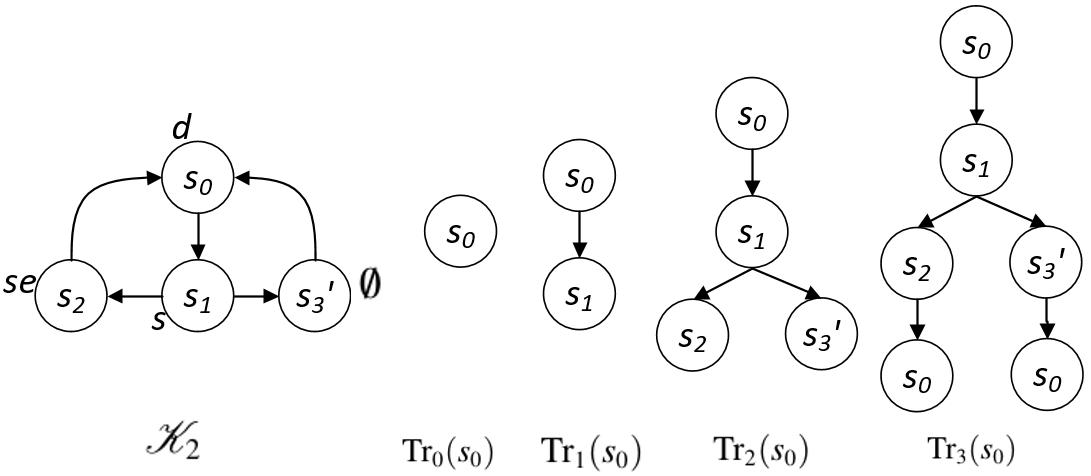
\includegraphics[width=10cm]{chapter05/NK2Tree2.png}
		\caption{初始结构$\mathcal{K}_2$(源于图\ref{Fig:chapter04:v1uv2})及其计算树示意图}\label{fig:K2Tree}
	\end{figure*}
	
	%\begin{figure*}[!htb]
	%	\centering
	%	% Requires \usepackage{graphicx}
	%	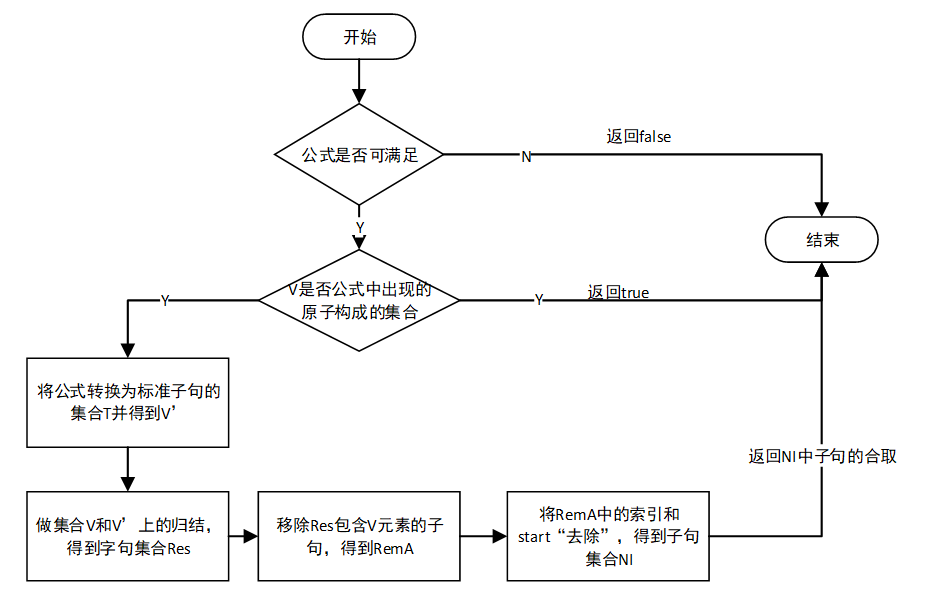
\includegraphics[width=15cm]{chapter04/frame.png}\\
	%	\caption{基于归结的遗忘的主要流程图}
	%	\label{Fig:chapter05:v1uv2}
	%\end{figure*}
	
\end{example}


下面的定理表示,特征公式描述了一个初始结构。此时,对系统结构的操作就可转换为对其特征公式的操作,如:下文中给定系统下的最弱充分条件计算。直观上,特征公式保持了给定初始结构在原子命题集$V$上的所有特性,即:具有$\overline{V}$-互模拟的两个初始结构关于$V$的特征公式逻辑等价。

\begin{theorem}\label{CF}
	令$V\subseteq \Ha$、$\Hm=(S,R,L,s_0)$且$\Hm'=(S',R', L',s_0')$,则:
	\begin{itemize}
		\item[(i)] $(\Hm',s_0') \models {\cal F}_V({\cal M},s_0)
		\text{ 当且仅当 }
		({\cal M},s_0) \lrto_{\overline V} ({\cal M}',s_0')$;
		
		\item[(ii)] 若$s_0 \lrto_{\overline V} s_0'$则${\cal F}_V(\Hm, s_0) \equiv {\cal F}_V(\Hm', s_0')$。
	\end{itemize}
	
\end{theorem}
\begin{proof}
	(i) 令${\cal F}_V(\Hm, s_0)$为$(\Hm, s_0)$关于$V$的特征公式。显然,$\IR({\cal F}_V(\Hm, s_0), \overline V)$。为了证明上述结论成立,首先证明$(\Hm, s_0) \models {\cal F}_V(\Hm, s_0)$。
	
	令$c={ch({\cal M},V)}$,由引理\ref{Bn:to:Tn}可知$(\Hm, s_0) \models {\cal F}_V(\Tr_c(s_0))$。下证特征公式里的另一部分,即:$(\Hm, s_0) \models \bigwedge_{s\in S} \ALL\GLOBAL\ G(\Hm, s)$,其中
	\[G(\Hm, s) = {\cal F}_V(\Tr_c(s)) \rto \left(\bigwedge_{(s,s_1) \in R} \EXIST \NEXT {\cal F}_V(\Tr_c(s_1))\right)\wedge \ALL \NEXT \left(\bigvee_{(s,s_1) \in R} {\cal F}_V(\Tr_c(s_1))\right).\]
	
	为此,下面证明$(\Hm, s_0) \models \ALL\GLOBAL\ G(\Hm, s)$。考虑下面两种情况:
	\begin{itemize}
		\item  若$(\Hm, s_0) \not \models {\cal F}_V(\Tr_c(s))$,显然$(\Hm, s_0) \models G(\Hm, s)$;
		\item 若$(\Hm, s_0) \models {\cal F}_V(\Tr_c(s))$:\\
		$(\Hm, s_0) \models {\cal F}_V(\Tr_c(s))$\\
		$\Rto$  $s_0 \lrto_{\overline V} s$ \hfill (引理\ref{div_s})
		
		$\forall (s, s_1)\in R$:\\
		$(\Hm, s_1) \models {\cal F}_V(\Tr_c(s_1))$  \hfill  ($s_1 \lrto_{\overline V} s_1$)\\
		$\Rto$ $(\Hm, s) \models \bigwedge_{(s,s_1)\in R}\EXIST \NEXT {\cal F}_V(\Tr_c(s_1))$\\
		$\Rto$ $(\Hm, s_0) \models$ $\bigwedge_{(s,s_1)\in R}\EXIST \NEXT {\cal F}_V(\Tr_c(s_1))$  \hfill ($\IR(\bigwedge_{(s,s_1)\in R}\EXIST \NEXT {\cal F}_V(\Tr_c(s_1)), \overline V)$, $s_0 \lrto_{\overline V} s$)
		
		$\forall (s, s_1) \in R$:\\
		$(\Hm, s_1) \models \bigvee_{(s, s_2)\in R}{\cal F}_V(\Tr_c(s_2))$\\
		$\Rto$ $(\Hm, s) \models \ALL \NEXT \left( \bigvee_{(s, s_2)\in R} {\cal F}_V(\Tr_c(s_2)) \right)$ \\
		$\Rto$ $(\Hm, s_0) \models$  $\ALL \NEXT \left( \bigvee_{(s, s_2)\in R} {\cal F}_V(\Tr_c(s_2)) \right)$   \hfill  ($\IR(\ALL \NEXT \left( \bigvee_{(s, s_2)\in R} {\cal F}_V(\Tr_c(s_2)) \right), \overline V)$, $s_0 \lrto_{\overline V} s$)\\
		$\Rto$ $(\Hm, s_0) \models G(\Hm, s)$。\\
		% where $s_i$ and $s_j$ are the successors of $s$.
	\end{itemize}
	
	对任意其它能从$s_0$可达的状态$s'$,都可以类似地证明$(\Hm,s')\models G(\Hm, s)$。
	因此,对任意$s\in S$,$(\Hm, s_0) \models \ALL\GLOBAL\ G(\Hm, s)$,从而$(\Hm, s_0) \models {\cal F}_V(\Hm, s_0)$。
	
	下面从两个方面证明(i)成立:
	
	$(\Lto)$ 证明:若$s_0 \lrto_{\overline V} s_0'$,则$(\Hm',s_0') \models {\cal F}_V(\Hm,s_0)$。因为$(\Hm, s_0) \models {\cal F}_V($ $\Hm, s_0)$且 $\IR($ ${\cal F}_V(\Hm, s_0), \overline V)$,由定理\ref{thm:V-bisimulation:EQ}可知
	$(\Hm',s_0') \models {\cal F}_V(\Hm,s_0)$。
	
	$(\Rto)$ 证明:若$(\Hm',s_0') \models {\cal F}_V(\Hm,s_0)$,则$s_0 \lrto_{\overline V} s_0'$。为此,下面证明对任意$n \geq 0$,$Tr_n(s_0) \lrto_{\overline V} Tr_n(s_0')$。
	
	
	\textbf{基始($n=0$):} 由特征公式的定义,显然$Tr_0(s_0) \equiv Tr_0(s_0')$成立。
	
	\textbf{归纳步骤($n>0$):} 假定对任意$k > 0$,都有$\Tr_k(s_0) \lrto_{\overline V} \Tr_k(s_0')$,下面证明$\Tr_{k+1}(s_0)$ $\lrto_{\overline V} \Tr_{k+1}(s_0')$。令$(s_0, s_1), (s_1, s_2)$, $\dots$, $(s_{k-1}, s_k) \in R$且$(s_0', s_1'), (s_1', s_2'), \dots, (s_{k-1}', s_k') \in R'$,即对于任意$0 \leq i \leq k-1$,$s_{i+1}$($s_{i+1}'$)是$s_i$($s_i'$)的直接后继状态。
	由归纳假设可知,只需证明$\Tr_1(s_k) \lrto_{\overline V} \Tr_1(s_k')$。
	
	(a) 由归纳假设可知$L(s_k) - \overline V = L'(s_k') - \overline V$。
	
	在讨论其它点时,首先考虑下面事实(\textbf{fact}):\\
	$(\Hm',s_0') \models {\cal F}_V(\Hm,s_0)$\\
	$\Rto$ $\forall s'\in S'$,$\forall s\in S$,\\ $(\Hm', s')\models {\cal F}_V(\Tr_c(s)) \rto$  $\left(\bigwedge_{(s,s_1)\in R} \EXIST \NEXT {\cal F}_V(\Tr_c(s_1))\right)\wedge \ALL \NEXT \left( \bigvee_{(s,s_1)\in R} {\cal F}_V(\Tr_c(s_1))\right)$  \\
	(I) $(\Hm', s_0') \models {\cal F}_V(\Tr_c(s_0)) \rto \left(\bigwedge_{(s_0, s_1) \in R} \EXIST \NEXT {\cal F}_V(\Tr_c(s_1))\right)$ $\wedge$ $\ALL \NEXT \left(\bigvee_{(s_0, s_1) \in R} {\cal F}_V(\Tr_c(s_1)) \right)$     \\
	(II) $(\Hm', s_0') \models {\cal F}_V(\Tr_c(s_0)))$  \hfill  (已知)\\
	(III) $(\Hm', s_0') \models \left(\bigwedge_{(s_0, s_1) \in R} \EXIST \NEXT {\cal F}_V(\Tr_c(s_1))\right)$ $\wedge$ $\ALL \NEXT \left(\bigvee_{(s_0, s_1) \in R} {\cal F}_V(\Tr_c(s_1)) \right)$  \hfill  ((I),(II))\\
	
	% It is apparent that $L'(s_0') - \overline V = L(s_0) - \overline V$;\\
	(b) 下证$\forall (s_k, s_{k+1}) \in R$,存在$(s_k', s_{k+1}') \in R'$,使得$L(s_{k+1}) - \overline V = L'(s_{k+1}') - \overline V$。\\
	(1) $(\Hm', s_0') \models \bigwedge_{(s_0, s_1) \in R} \EXIST \NEXT {\cal F}_V(\Tr_c(s_1))$  \hfill  (III)\\
	(2) $\forall (s_0, s_1) \in R$,$\exists (s_0', s_1') \in R'$,使得 $(\Hm', s_1') \models {\cal F}_V(\Tr_c(s_1))$  \hfill  (1)\\
	(3) $\Tr_c(s_1) \lrto_{\overline V} \Tr_c(s_1')$  \hfill  ((2), 引理\ref{Bn:to:Tn}) \\
	(4) $L(s_1) - \overline V = L'(s_1') - \overline V$  \hfill   ((3), $c \geq 0)$\\
	(5) $(\Hm', s_1') \models {\cal F}_V(\Tr_c(s_1)) \rto \left(\bigwedge_{(s_1,s_2)\in R} \EXIST \NEXT {\cal F}_V(\Tr_c(s_2))\right) \wedge \ALL \NEXT \left(\bigvee_{(s_1,s_2)\in R} {\cal F}_V(\Tr_c(s_2))\right)$     \hfill  \textbf{(fact)}\\
	(6) $(\Hm', s_1') \models \left(\bigwedge_{(s_1,s_2)\in R} \EXIST \NEXT {\cal F}_V(\Tr_c(s_2))\right) \wedge \ALL \NEXT \left(\bigvee_{(s_1,s_2)\in R} {\cal F}_V(\Tr_c(s_2))\right)$ \hfill ((2), (5))\\
	%(7) $\dots \dots$ \\
	(7) $(\Hm', s_k') \models \left(\bigwedge_{(s_k,s_{k+1})\in R} \EXIST \NEXT {\cal F}_V(\Tr_c(s_{k+1}))\right) \wedge \ALL \NEXT \left(\bigvee_{(s_k,s_{k+1})\in R} {\cal F}_V(\Tr_c(s_{k+1}))\right)$       \hfill (与(6)类似)\\
	(8) $\forall (s_k, s_{k+1}) \in R$,$\exists (s_k', s_{k+1}') \in R'$,使得$(\Hm', s_{k+1}') \models {\cal F}_V(\Tr_c(s_{k+1}))$  \hfill  (7)\\
	(9) $\Tr_c(s_{k+1}) \lrto_{\overline V} \Tr_c(s_{k+1}')$    \hfill ((8), 引理\ref{Bn:to:Tn}) \\
	(10) $L(s_{k+1}) - \overline V = L'(s_{k+1}') - \overline V$  \hfill   ((9), $c \geq 0)$\\
	
	(c) 下证$\forall (s_k', s_{k+1}') \in R'$,存在$(s_k, s_{k+1})\in R$,使得$L(s_{k+1}) - \overline V = L'(s_{k+1}') - \overline V$。\\
	(1) $(\Hm', s_k') \models \ALL \NEXT \left(\bigvee_{(s_k,s_{k+1})\in R} {\cal F}_V(\Tr_c(s_{k+1}))\right)$  \hfill (上面的(7))\\
	(2) $\forall (s_k', s_{k+1}') \in R'$,$\exists (s_k, s_{k+1}) \in R$,使得$(\Hm', s_{k+1}') \models {\cal F}_V(\Tr_c(s_{k+1}'))$  \hfill (1) \\
	(3) $\Tr_c(s_{k+1}) \lrto_{\overline V} \Tr_c(s_{k+1}')$    \hfill ((2), 引理\ref{Bn:to:Tn}) \\
	(4) $L(s_{k+1}) - \overline V = L'(s_{k+1}') - \overline V$  \hfill   ((3), $c \geq 0)$\\
	
	(ii) 由引理\ref{lem:Vb:TrFormula:Equ}和\ref{div_s} 易得。
	
\end{proof}



\section{最弱充分条件}
\label{chapter04:sec:snc}
这部分介绍如何使用遗忘理论计算最强必要条件和最弱充分条件。
直观地说,最强必要条件指最一般的结果(the most general consequence),最弱充分条件指最特殊的诱因(the most specific abduction)。
下面给出其形式化定义,本章所说的公式指$\CTL$公式,且这章所有的定义和结论都可以平凡地移到$\mu$-句子下。
\begin{definition}[充分和必要条件]\label{def:NC:SC}
	给定两个公式$\varphi$和$\psi$,$V \subseteq \Var(\varphi)$,$q\in\Var(\varphi)- V$
	和$\Var(\psi)$ $\subseteq V$。
	\begin{itemize}
		\item 若$\varphi \models q \rto \psi$,则称$\psi$是$q$在$V$和$\varphi$上的{\em 必要条件(necessary condition,NC)};
		\item 若$\varphi \models \psi\rto q$,则称$\psi$是$q$在$V$和$\varphi$上的{\em 充分条件(sufficient condition,SC)};
		\item 若$\psi$是$q$在$V$和$\varphi$上的必要条件,且对于任意$q$ 在$V$和$\varphi$上的必要条件$\psi'$,都有$\varphi\models\psi\rto\psi'$,则称$\psi$是$q$在$V$和$\varphi$上的{\em 最强必要条件(strongest necessary condition,SNC)};
		\item 若$\psi$是$q$在$V$和$\varphi$上的充分条件,且对于任意$q$ 在$V$和$\varphi$上的充分条件$\psi'$,都有$\varphi\models\psi'\rto\psi$,则称$\psi$是$q$在$V$和$\varphi$上的{\em 最弱充分条件(weakest sufficient condition, WSC)}。
	\end{itemize}
\end{definition}

从上述定义可以看出,SNC(WSC)是$q$在$V$和$\varphi$上的NC(SC)中最强(最弱)的一个。此外,如果公式$\psi$和$\psi'$都是$q$在$V$和$\varphi$上的SNC (WSC),则$\psi \equiv \psi'$。
下面的命题表明SNC和WSC是一对对偶概念。

\begin{proposition}[对偶性]\label{dual}
	令$V$、$q$、$\varphi$和$\psi$为定义\ref{def:NC:SC}出现的符号。
	则$\psi$是$q$在$V$和$\varphi$上的SNC(WSC)当且仅当$\neg \psi$是$\neg q$ 在$V$和$\varphi$上的WSC(SNC)。
\end{proposition}
\begin{proof}
	(i) 假定$\psi$是$q$在$V$和$\varphi$ 上的SNC,$\psi'$是$\neg q$在$V$和$\varphi$上SC。
	
	$\varphi \models q \rto \psi$ \\
	$\Rto$ $\varphi \models \neg \psi \rto \neg q$。
	
	这表明$\neg \psi$是$\neg q$在$V$和$\varphi$的SC。
	%Suppose $\psi'$ is any other SC of $\neg q$, and
	%We now show $\varphi \models \psi' \rto \neg \psi$.
	
	$\varphi \models \psi' \rto \neg q$\\
	$\Rto$ $\varphi \models q \rto \neg \psi'$,即:$\neg \psi'$是$q$在$V$和$\varphi$上的NC\\
	$\Rto$ $\varphi \models \psi \rto \neg \psi'$ \hfill (假设)\\
	$\Rto$ $\varphi \models \psi' \rto \neg \psi$。
	
	另一个方向可以类似地证明。
	%      (i) Suppose $\psi$ is the SNC of $q$. Then $\varphi \models q \rto \psi$, and then $\varphi \models \neg \psi \rto \neg q$, i.e., $\neg \psi$ is an
	% SC of $\neg q$. Suppose $\psi'$ is any other SC of $\neg q$: $\varphi \models \psi' \rto \neg q$. Then $\varphi \models q \rto \neg \psi'$, i.e., $\neg \psi'$ is an NC of $q$ on $V$ under $\varphi$.
	% Therefore, $\varphi \models \psi \rto \neg \psi'$ by assumption, and then $\varphi \models \psi' \rto \neg \psi$. This proves that $\neg \psi$ is the WSC of $\neg q$.
	% The proof of the other part of the proposition is similar.
	
	(ii) 可以类似SNC的情形证明。
\end{proof}


在定义\ref{def:NC:SC}中,用公式$\alpha$ 替换$q$,$V\subseteq \Var(\alpha) \cup \Var(\phi)$,则为公式的最强必要条件和最弱充分条件的定义。
下面的命题表明了原子命题的充分(必要)条件与公式的充分(必要)条件之间的关系:通过计算原子命题的充分(必要)条件来计算公式的充分(必要)条件。



\begin{proposition}\label{formulaNS_to_p}
	给定公式$\Gamma$和$\alpha$, $V \subseteq \Var(\alpha) \cup \Var(\Gamma)$,$q$是不出现在$\Gamma$和$\alpha$中的原子命题。
	$\varphi$是集合$V$上的公式,则$\varphi$是$\alpha$在$V$和$\Gamma$上的SNC(WSC) 当且仅当$\varphi$是$q$在$V$ 和$\Gamma'$上的SNC(WSC),其中$\Gamma' = \Gamma \cup \{q \lrto \alpha\}$。
\end{proposition}
\begin{proof}
	这里证明SNC的情形,WSC的情形可以类似地证明。
	记$\emph{SNC}(\varphi,\beta,V,\Gamma)$为$\varphi$是$\beta$ 在 $V$和$\Gamma$上的SNC,$\emph{NC}(\varphi,\beta,V,\Gamma)$为$\varphi$是$\beta$在$V$和 $\Gamma$上的NC。
	
	($\Rto$) 下证$\emph{SNC}(\varphi,\alpha,V,\Gamma)\Rto \emph{SNC}(\varphi,q,V,\Gamma')$。假设$\varphi'$是$q$在$V$和$\Gamma'$上的NC。
	
	$\Gamma \models \alpha \rto \varphi$ \hfill  (已知)\\
	$\Rto$ $\Gamma \wedge (q \lrto \alpha) \models \alpha \rto \varphi$\\
	$\Rto$ $\Gamma' \models q \rto \varphi$  \hfill ($q \equiv \alpha$)
	
	$\Gamma' \models q \rto \varphi'$ \hfill (假设) \\
	$\Rto$ $\Gamma' \models \alpha \rto \varphi'$ \hfill ($q \equiv \alpha$)\\
	$\Rto$ $\Muforget(\Gamma', \{q\}) \models \alpha \rto \varphi'$ \hfill ($\IR(\alpha \rto \varphi', \{q\})$, $(\PP)$)\\
	$\Rto$ $\Gamma \models \alpha \rto \varphi'$ \hfill  (引理~\ref{lem:KF:eq})\\
	$\Rto$ $\Gamma \models \varphi \rto \varphi'$ \hfill  (已知: $\emph{SNC}(\varphi,\alpha,V,\Gamma)$)\\
	$\Rto$ $\Gamma' \models \varphi \rto \varphi'$.
	
	总之,$\varphi$是$q$在$V$和$\Gamma'$上的NC,且对任意$q$在$V$和$\Gamma'$上的NC$\varphi'$,有$\Gamma' \models \varphi \rto \varphi'$。因此, $\emph{SNC}(\varphi,q,V,\Gamma')$。
	
	($\Lto$) 下证$\emph{SNC}(\varphi,q,V,\Gamma')\Rto \emph{SNC}(\varphi,\alpha,V,\Gamma)$。 假定$\varphi'$是$\alpha$在$V$和$\Gamma$ 上的NC。
	
	$\Gamma' \models q \rto \varphi$ \hfill  (已知)\\
	$\Rto$  $\Gamma' \models \alpha \rto \varphi$ \hfill  ($q \equiv \alpha$)\\
	$\Rto$  $\Muforget(\Gamma', \{q\}) \models \alpha \rto \varphi$ \hfill ($\IR(\alpha \rto \varphi, \{q\})$, $(\PP)$)\\
	$\Rto$ $\Gamma \models \alpha \rto \varphi$ \hfill  (引理~\ref{lem:KF:eq})
	
	$\Gamma \models \alpha \rto \varphi'$ \hfill  (假设)\\
	$\Rto$ $\Gamma' \models \alpha \rto \varphi'$ \\
	$\Rto$ $\Gamma' \models q \rto \varphi'$ \hfill  ($q \equiv \alpha$)\\
	$\Rto$ $\Gamma' \models \varphi \rto \varphi'$ \hfill (已知:$\emph{SNC}(\varphi,q,V,\Gamma')$)\\
	$\Rto$ $\Muforget(\Gamma', \{q\}) \models \varphi \rto \varphi'$ \hfill ($\IR(\varphi \rto \varphi', \{q\})$, $(\PP)$)\\
	$\Rto$ $\Gamma \models \varphi \rto \varphi'$ \hfill (引理~\ref{lem:KF:eq})
	
	总之,$\varphi$是$\alpha$在$V$和$\Gamma$上的NC,且对任意$\alpha$在$V$和$\Gamma$上的NC$\varphi'$,有$\Gamma \models \varphi \rto \varphi'$。因此, $\emph{SNC}(\varphi,\alpha,V,\Gamma)$。
\end{proof}


%为了对给定原子命题集合下公式的最弱充分条件有个直观的认识,下面给出一个简单的例子。
%下面的例子给出了关于给定原子命题集合下的公式的最弱充分条件的具体体现。

\begin{example}[例\ref{exam:vB}的延续]\label{examp:WSC}
	本例来源于图\ref{exam:vB}中的初始结构${\cal K}_2$。令$\psi = \EXIST \NEXT(s \wedge (\EXIST \NEXT se \vee \EXIST \NEXT \neg d))$、$\varphi = \EXIST \NEXT(s \wedge \EXIST \NEXT \neg d)$、$\Ha =\{d, s, se\}$和$V = \{s, d\}$。下面证明$\varphi$是$\psi$在$V$和${\cal K}_2$上的WSC:
	\begin{itemize}
		\item[(i)] 由已知有$\varphi \models \psi$和$\Var(\varphi) \subseteq V$。此外,$(\Hm, s_0) \models \varphi \wedge \psi$,因此${\cal K}_2 \models \varphi \rto \psi$,即:$\varphi$是$\psi$在$V$和${\cal K}_2$上的SC;
		\item[(ii)] 下证“对任意$\psi$ 在$V$和${\cal K}_2$上的SC $\varphi'$ 都有${\cal K}_2 \models \varphi' \rto \varphi$”。易知若${\cal K}_2 \not \models \varphi'$,则${\cal K}_2\models \varphi' \rto \varphi$。
		假设${\cal K}_2 \models \varphi'$。由$\varphi'$是$\psi$在$V$ 和${\cal K}_2$上的SC可知$\varphi' \models \EXIST \NEXT(s \wedge \phi)$,其中$\phi$是使得$\phi\models \EXIST \NEXT se \vee \EXIST \NEXT \neg d$成立的公式。又$\IR(\varphi', \overline V)$,所以$\phi \models \EXIST \NEXT \neg d$。因此,$\varphi' \models \varphi$且${\cal K}_2 \models \varphi' \rto \varphi$。
	\end{itemize}
\end{example}


如何使用遗忘计算SNC(WSC)是本章讨论的关键问题。下面首先给出其理论基础,然后再做直观的解释。


\begin{theorem}\label{thm:SNC:WSC:forget}
	给定公式$\varphi$、原子命题集$V\subseteq\Var(\varphi)$和原子命题$q\in\Var(\varphi)- V$。
	\begin{itemize}
		\item[(i)] $\CTLforget (\varphi \land q$, $(\Var(\varphi) \cup \{q\}) - V)$是$q$在$V$和$\varphi$上的SNC;
		\item[(ii)]  $\neg\CTLforget (\varphi \land \neg q$, $(\Var(\varphi) \cup \{q\}) - V)$是$q$在$V$和$\varphi$上的WSC。
	\end{itemize}
\end{theorem}
\begin{proof}
	(i) 令${\cal F}=\CTLforget(\varphi \wedge q, (\Var(\varphi) \cup \{q\})- V)$。
	
	
	“NC”部分:由遗忘的定义可知$\varphi \wedge q \models {\cal F}$。因此,$\varphi\models q \rto {\cal F}$,即:${\cal F}$是$q$在$V$ 和$\varphi$ 上的NC。
	
	“SNC”部分:假设$\psi'$为$q$在$V$和$\varphi$上的任意NC,即:$\varphi\models q \rto \psi'$。由定理\ref{thm:V-bisimulation:EQ} 和 $\emph{IR}(\psi', (\Var(\varphi) \cup \{q\})- V)$可知,若$\varphi \wedge q \models \psi'$,则${\cal F} \models \psi'$。
	由假设可知$\varphi\models q \rto \psi'$,所以$\varphi \wedge {\cal F} \models \psi'$,因此$\varphi \models {\cal F} \rto \psi'$。
	
	由上面两部分可知,${\cal F}$是$q$在$V$和$\varphi$上的SNC。
	
	(ii) 令${\cal F}=\neg \CTLforget(\varphi \wedge \neg q, (\Var(\varphi) \cup \{q\})- V)$。
	由命题\ref{dual}可知,对任意命题$q'$,$\CTLforget$ $(\varphi \wedge q', (\Var(\varphi) \cup \{q'\})- V)$是$q'$ 在$V$和$\varphi$上的SNC,当且仅当
	$\neg \CTLforget(\varphi \wedge q', (\Var(\varphi) \cup \{q'\})- V)$是$\neg q'$在$V$和$\varphi$上的WSC。
	由(i)可知$\CTLforget(\varphi \wedge q', (\Var(\varphi) \cup \{q'\})- V)$是$q'$在$V$和$\varphi$上的SNC,所以$\neg \CTLforget(\varphi \wedge q', (\Var(\varphi) \cup \{q'\})- V)$是$\neg q'$在$V$和$\varphi$上的WSC。令$q=\neg q'$,可得${\cal F}$是 $q$在 $V$ 和 $\varphi$上的WSC。
\end{proof}

令${\cal F}=\CTLforget(\varphi \wedge q, (\Var(\varphi) \cup \{q\})- V)$。上面的定理可以直观地解释如下:由遗忘理论的定义可知$\varphi \wedge q \models {\cal F}$,这说明
${\cal F}$是 $q$在 $V$和$\varphi$上的NC;对任意与$(\Var(\varphi) \cup \{q\})- V$无关的公式$\psi$,若$\varphi \wedge q \models \psi$,则由表达性定理可知${\cal F} \models \psi$。

值得注意的是,定理~\ref{thm:SNC:WSC:forget}中,当考虑的公式为$\mu$-公式时,要求出现在$\varphi$中的变元都包含在$V$中。

由第\ref{chapter05}章可知,任意有限的初始结构都能由一个$\CTL$公式表示,所以由上面的定理自然地就能得到给定有限初始结构下的SNC和WSC。
\begin{corollary}\label{thm:inK:SNC}
	令${\cal K}= (\Hm, s_0)$为初始结构,其中$\Hm=(S,R,L,s_0)$为有限原子命题集$\Ha$上的初始-Kripke结构,$V \subseteq \Ha$且$q\in V' = \Ha - V$。 则:
	\begin{itemize}
		\item[(i)] $\CTLforget({\cal F}_{\Ha}({\cal K}) \wedge q, V')$是$q'$在$V$和${\cal K}$上的SNC;
		\item[(ii)] $\neg \CTLforget({\cal F}_{\Ha}({\cal K}) \wedge \neg q, V')$是$q'$在$V$和${\cal K}$上的WSC。
	\end{itemize}
\end{corollary}

\begin{example}[例1的延续]
	\label{exam:SNCandWSC}
令$\Ha=\{d,se,sp,s\}$和$V=\{d,se\}$,求$s$在$V$和初始结构${\cal K} = (\Hm,s_0)$ 上的WSC,其中$\Hm$为例~\ref{car_manufacturing}中初始状态为$s_0$的汽车制造企业模型结构。

由定理~\ref{thm:inK:SNC}可知,$s$在$V$ 和初始结构${\cal K} = (\Hm,s_0)$上的WSC 为$\neg \CTLforget({\cal F}_{\Ha}({\cal K}) \wedge \neg s, \{s\}$ $\cup \{sp\})$。
\begin{align*}
	&	\CTLforget({\cal F}_{\Ha}({\cal K}) \wedge \neg s, \{s\} \cup \{sp\})\\
	&	\equiv \CTLforget(\CTLforget({\cal F}_{\Ha}({\cal K}) \wedge \neg s, \{sp\}), \{s\})\\
	&	\equiv \CTLforget(\CTLforget({\cal F}_{\Ha}({\cal K}), \{sp\})\wedge \neg s, \{s\}).
\end{align*}

${\cal K}_1 \models \CTLforget({\cal F}_{\Ha}({\cal K}), \{sp\})$\\
$\LRto$ 存在${\cal K}_1' \lrto_{\{sp\}} {\cal K}_1$,使得${\cal K}_1' \models {\cal F}_{\Ha}({\cal K})$和\\
$\LRto$ 存在${\cal K}_1' \lrto_{\{sp\}} {\cal K}_1$,使得${\cal K}_1' \lrto_{\emptyset} {\cal K}$\\
$\LRto$ 存在${\cal K}_1' \lrto_{\{sp\}} {\cal K}$和${\cal K}_1' \models {\cal F}_{V\cup \{s\}}({\cal K})$ \hfill (定理~\ref{CF})\\
$\LRto$ ${\cal K}_1 \models {\cal F}_{V\cup \{s\}}({\cal K})$。

由此可知,$ \CTLforget({\cal F}_{\Ha}({\cal K}), \{sp\}) \equiv {\cal F}_{V\cup \{s\}}({\cal K})$。所以要计算$\neg \CTLforget({\cal F}_{\Ha}({\cal K}) \wedge \neg s,$ $\{s\}\cup \{sp\})$,只需计算$\neg \CTLforget({\cal F}_{V\cup \{s\}}({\cal K})\wedge \neg s, \{s\})$。令$V' = V \cup \{s\} = \{d,se,s\}$,则$\overline{V'} = \{sp\}$。


易知,除了$s_2$和$s_4$是$\overline{V'}$-互模拟的以外,其余都是$V'$-可区分的,且$\dis_{V'}(\Hm, s_i, s_j, 0)$,其中$i\not =j$且$i$和$j$不能同时分别取值2和4。
因此,可以计算$\Hm$关于$V'$的特征数为:
$$ch(\Hm, V')=\max\{k\mid s,s'\in S \text{ 且 } \dis_{V'}({\cal M},s,s',k)\} = 0\hbox{。}$$


所以,可以由以下步骤计算${\cal K}_2$关于$V$的特征公式:
\begin{align*}
	{\cal F}_{V'}(\Tr_0(s_0)) &= d \wedge \neg se \wedge \neg s, \qquad \qquad \qquad \qquad \quad {\cal F}_{V'}(\Tr_0(s_1)) = \neg d \wedge \neg se \wedge s, \\
	{\cal F}_{V'} (\Tr_0(s_2)) &= {\cal F}_{V'} (\Tr_0(s_4)) = \neg d \wedge se \wedge \neg s,  \qquad  {\cal F}_{V'}(\Tr_0(s_3) = \neg d \wedge \neg se\wedge \neg s,\\
	{\cal F}_{V'}(\Hm, s_0)& \equiv d \wedge \neg se \wedge \neg s \wedge \\
	& \ALL \GLOBAL(d \wedge \neg se \wedge \neg s \rto \ALL\NEXT(\neg d \wedge \neg se \wedge s))\wedge \\
	& \ALL \GLOBAL(\neg d \wedge \neg se \wedge s \rto [\ALL\NEXT((\neg d \wedge se \wedge \neg s) \vee (\neg d \wedge \neg se\wedge \neg s)) \wedge\\ &\EXIST\NEXT(\neg d \wedge se \wedge \neg s) \wedge \EXIST\NEXT (\neg d \wedge \neg se\wedge \neg s)]) \wedge\\
	& \ALL \GLOBAL(\neg d \wedge \neg se\wedge \neg s \rto \ALL\NEXT(d \wedge \neg se \wedge \neg s)) \wedge\\
	& \ALL \GLOBAL(\neg d \wedge se \wedge \neg s \rto \ALL\NEXT(d \wedge \neg se \wedge \neg s)).
\end{align*}
令:
\begin{align*}
	\varphi_1&  = d \wedge \neg se \wedge \neg s \rto \ALL\NEXT(\neg d \wedge \neg se \wedge s)\equiv \neg d \vee se \vee s \vee \ALL\NEXT(\neg d \wedge \neg se \wedge s),\\
	\varphi_2& = \neg d \wedge \neg se \wedge s \rto \ALL\NEXT(\neg d \wedge se \wedge \neg s) \equiv d \vee  se \vee \neg s \vee\\
	& [\ALL\NEXT((\neg d \wedge se \wedge \neg s) \vee (\neg d \wedge \neg se\wedge \neg s)) \wedge\EXIST\NEXT(\neg d \wedge se \wedge \neg s) \wedge \EXIST\NEXT (\neg d \wedge \neg se\wedge \neg s)],\\
	\varphi_3 &=\neg d \wedge \neg se\wedge \neg s \rto \ALL\NEXT(d \wedge \neg se \wedge \neg s)\equiv d \vee se \vee s \vee \ALL\NEXT(d \wedge \neg se \wedge \neg s),\\
	\varphi_4 &= \neg d \wedge se \wedge \neg s \rto \ALL\NEXT(d \wedge \neg se \wedge \neg s)\equiv d \vee \neg se \vee s \vee \ALL\NEXT(d \wedge \neg se \wedge \neg s).
\end{align*}
此外,令
\begin{align*}
	& \psi_1 = \neg d \vee se \vee s && \psi_2 = d \vee  se \vee \neg s \\
	& \psi_3 = d \vee se \vee s && \psi_4 = d \vee \neg se \vee s\\
	& \alpha_1 = \ALL\NEXT(\neg d \wedge \neg se \wedge s) && \alpha_2 = \ALL\NEXT((\neg d \wedge se \wedge \neg s) \vee (\neg d \wedge \neg se\wedge \neg s))\\
	& \alpha_3 = \EXIST\NEXT(\neg d \wedge se \wedge \neg s) \wedge \EXIST\NEXT (\neg d \wedge \neg se\wedge \neg s) && \alpha_4 = \ALL\NEXT(d \wedge \neg se \wedge \neg s)\\
	& \alpha_5 = \ALL\NEXT(d \wedge \neg se \wedge \neg s) && \psi = d \wedge \neg se \wedge \neg s.
\end{align*}
则,
\begin{align*}
	& \psi \wedge \varphi_1 \wedge \varphi_2 \wedge \varphi_3\wedge \varphi_4
	\equiv (\psi \wedge \psi_1 \wedge \psi_2 \wedge \psi_3 \wedge \psi_4) \vee (\psi \wedge \psi_1 \wedge \psi_2 \wedge \psi_3 \wedge \alpha_5) \vee\\
	& (\psi \wedge \psi_1 \wedge \psi_2 \wedge \alpha_4 \wedge \psi_4) \vee (\psi \wedge \psi_1 \wedge \psi_2 \wedge \alpha_4 \wedge \alpha_5) \vee\\
	& (\psi \wedge \psi_1 \wedge \alpha_2 \wedge \alpha_3 \wedge \psi_3 \wedge \psi_4) \vee (\psi \wedge \psi_1 \wedge \alpha_2 \wedge \alpha_3 \wedge \psi_3 \wedge \alpha_4) \vee \\
	& (\psi \wedge \psi_1 \wedge \alpha_2 \wedge \alpha_3 \wedge \alpha_4 \wedge \psi_4) \vee (\psi \wedge \psi_1 \wedge \alpha_2 \wedge \alpha_3 \wedge \alpha_4 \wedge \alpha_5) \vee\\
	& (\psi \wedge \alpha_1 \wedge \psi_2 \wedge \psi_3 \wedge \psi_4) \vee (\psi \wedge \alpha_1 \wedge \psi_2 \wedge \psi_3 \wedge \alpha_5)\vee\\
	& (\psi \wedge \alpha_1 \wedge \psi_2 \wedge \alpha_4 \wedge \psi_4) \vee (\psi \wedge \alpha_1 \wedge \psi_2 \wedge \alpha_4 \wedge\alpha_5)\vee \\
	& (\psi \wedge \alpha_1 \wedge \alpha_2 \wedge \alpha_3 \wedge \psi_3 \wedge \psi_4) \vee (\psi \wedge \alpha_1 \wedge \alpha_2 \wedge \alpha_3\wedge \psi_3 \wedge \alpha_5) \vee \\
	& (\psi \wedge \alpha_1 \wedge \alpha_2 \wedge \alpha_3 \wedge \alpha_4 \wedge \psi_4) \vee (\psi \wedge \alpha_1 \wedge \alpha_2 \wedge \alpha_3 \wedge \alpha_4 \wedge \alpha_5).\\
	\\
	%\end{align*}
	%\begin{align*}
	& \varphi_1 \wedge \varphi_2 \wedge \varphi_3\wedge \varphi_4
	\equiv (\psi_1 \wedge \psi_2 \wedge \psi_3 \wedge \psi_4) \vee (\psi_1 \wedge \psi_2 \wedge \psi_3 \wedge \alpha_5) \vee\\
	& (\psi_1 \wedge \psi_2 \wedge \alpha_4 \wedge \psi_4) \vee (\psi_1 \wedge \psi_2 \wedge \alpha_4 \wedge \alpha_5) \vee\\
	& (\psi_1 \wedge \alpha_2 \wedge \alpha_3 \wedge \psi_3 \wedge \psi_4) \vee ( \psi_1 \wedge \alpha_2 \wedge \alpha_3 \wedge \psi_3 \wedge \alpha_4) \vee \\
	& ( \psi_1 \wedge \alpha_2 \wedge \alpha_3 \wedge \alpha_4 \wedge \psi_4) \vee ( \psi_1 \wedge \alpha_2 \wedge \alpha_3 \wedge \alpha_4 \wedge \alpha_5) \vee\\
	& (\alpha_1 \wedge \psi_2 \wedge \psi_3 \wedge \psi_4) \vee ( \alpha_1 \wedge \psi_2 \wedge \psi_3 \wedge \alpha_5)\vee\\
	& (\alpha_1 \wedge \psi_2 \wedge \alpha_4 \wedge \psi_4) \vee ( \alpha_1 \wedge \psi_2 \wedge \alpha_4 \wedge\alpha_5)\vee \\
	& (\alpha_1 \wedge \alpha_2 \wedge \alpha_3 \wedge \psi_3 \wedge \psi_4) \vee (\alpha_1 \wedge \alpha_2 \wedge \alpha_3\wedge \psi_3 \wedge \alpha_5) \vee \\
	& ( \alpha_1 \wedge \alpha_2 \wedge \alpha_3 \wedge \alpha_4 \wedge \psi_4) \vee ( \alpha_1 \wedge \alpha_2 \wedge \alpha_3 \wedge \alpha_4 \wedge \alpha_5).
\end{align*}
所以,
\begin{align*}
	&\neg \CTLforget({\cal F}_{V\cup \{s\}}({\cal K})\wedge \neg s, \{s\}) \\
	& \equiv \neg \CTLforget({\cal F}_{V\cup \{s\}}({\cal K}), \{s\})\\
	& \equiv \neg \CTLforget(\psi \wedge \ALL \GLOBAL(\varphi_1 \wedge \varphi_2 \wedge \varphi_3\wedge \varphi_4),\{s\})\\	
	& \equiv \neg(\CTLforget(\psi \wedge \varphi_1 \wedge \varphi_2 \wedge \varphi_3\wedge \varphi_4, \{s\}) \wedge \ALL \GLOBAL \CTLforget(\varphi_1 \wedge \varphi_2 \wedge \varphi_3\wedge \varphi_4, \{s\}))\\
	& \equiv  \neg \bigg(\Big(d \vee \big((d\vee se) \wedge \ALL\NEXT(d \wedge \neg se)\big) \vee \big((d \vee se \vee \ALL\NEXT \neg d) \wedge \EXIST\NEXT(\neg d \wedge se) \wedge \EXIST\NEXT(\neg d \wedge \neg se)\big) \\
	& \vee (d \wedge \ALL\NEXT(\neg d \wedge \neg se)) \vee \big((d\vee \neg se) \wedge \EXIST\NEXT\neg d\big) \Big) \wedge\\
	& \ALL \GLOBAL\Big(\big((d \vee se) \wedge \ALL\NEXT(d \wedge \neg se)\big) \vee \big(\ALL\NEXT \neg d \wedge \EXIST\NEXT(\neg d \wedge se) \wedge\\
	& \EXIST\NEXT(\neg d \wedge \neg se)\big) \vee \big((d\vee se) \wedge \ALL\NEXT(\neg d \wedge \neg se)\big) \vee \EXIST\NEXT \neg d\Big)
	\bigg).
\end{align*}
\end{example}


\section{知识更新}\label{chapter04:sec:update}
本小节介绍遗忘的另一个应用:知识更新(Knowledge update)。
具体说来,本节将使用遗忘定义知识更新,使得用这种方式定义的知识更新满足下面由Katsuno和Mende- lzon提出的基本条件\cite{katsuno91mendelzon}:
\begin{itemize}
	\item (U1)  $\Gamma \diamond \varphi \models \varphi$;
	\item (U2) 若$\Gamma \models \varphi$,则$\Gamma \diamond \varphi \equiv \Gamma$;
	\item (U3) 若$\Gamma$和$\varphi$ 都是可满足的,则$\Gamma \diamond \varphi$是可满足的;
	\item (U4) 若$\Gamma_1\equiv \Gamma_2$且$\varphi_1 \equiv \varphi_2$,则$\Gamma_1 \diamond \varphi_1 \equiv \Gamma_2 \diamond \varphi_2$;
	\item (U5) $(\Gamma \diamond \varphi) \wedge \psi \models \Gamma \diamond(\varphi \wedge \psi)$;
	\item (U6) 若$\Gamma \diamond \varphi \models \psi$且$\Gamma \diamond \psi \models \varphi$,则$\Gamma \diamond \varphi \equiv \Gamma \diamond \psi$;
	\item (U7) 若$\Gamma$有唯一一个模型,则$(\Gamma \diamond \varphi) \wedge (\Gamma \diamond \psi) \models \Gamma \diamond (\varphi \vee \psi)$;
	\item (U8) $(\Gamma_1 \vee \Gamma_2) \diamond \varphi \equiv (\Gamma_1 \diamond \varphi) \vee  (\Gamma_2 \diamond \varphi)$。
\end{itemize}
其中,$\diamond$为知识更新操作,$\varphi \diamond \psi$表示用$\psi$更新$\varphi$得到的结果。

本小节假设所有初始结构都是有限的,即:状态来源于有限状态空间且$\Ha$为有限原子命题集。

%下面定理显然成立:
%\begin{theorem}\label{thm:initModel}
%	给定公式$\varphi$和原子命题集$V \subseteq \cal A$。存在一个公式$\psi$使得:
%	\[
%	(\Hm,s_0) \models \psi \mbox{ 当且仅当存在 } (\Hm',s_0')\in\Mod(\varphi) \mbox{ 使得 } (\Hm,s_0) \lrto_V (\Hm',s_0') % \mbox{ and } \Hm' \models \phi.
%	\]
%	其中$(\Hm,s_0)$和$(\Hm',s_0')$都是有限的初始结构。
%\end{theorem}
%\begin{proof}
%	令$\psi=\Muforget(\varphi, V)$(或$\psi=\CTLforget(\varphi, V)$)。由遗忘的定义可知,对任意的${\cal K} \models \psi$存在一个${\cal K}' \models \varphi$使得${\cal K} \lrto_V {\cal K}'$,且对每一个${\cal K}' \in \Mod(\varphi)$都有${\cal K}' \models \psi$。
%	此时,容易证明对任意的有限初始结构${\cal K}$,若${\cal K} \models \psi$,则存在一个${\cal K}'$使得${\cal K}' \models \varphi$且${\cal K} \lrto_V {\cal K}'$。
%	
%	此外,对任意的${\cal K}' \in \Mod(\varphi)$,由(\W)可知存在${\cal K}' \models \psi$。又${\cal K} \lrto_V {\cal K}'$,所以$\Hm \models \psi$。
%\end{proof}


%定理\ref{thm:initModel}表明模型结构被限制到有限初始结构下的$\mu$-演算下遗忘理论也是封闭的。
由第\ref{chapter05}章可知,任意$\Ha$上的有限初始结构$\Hm$(为了简化符号,本节用初始Kripke结构$\Hm$代替初始结构$(\Hm,s_0)$)都能用一个$\CTL$公式——特征公式${\cal F}_{\Ha}(\Hm)$来表示。%,此公式也是$\mu$-句子。
给定公式$\varphi$和$\psi$,$V_{min}\subseteq \Ha$为使得$\CTLforget(\varphi, V_{min}) \wedge \psi$可满足的极小子集。
%,记$\varphi = \CTLforget({\cal F}_{\Ha}({\cal K}), V_{min})$,其中$V_{min} \subseteq \Ha$是使得$\varphi$ 可满足的极小子集。
此外,记
$$\bigcup_{V_{min}\subseteq \Ha} \Mod(\CTLforget({\cal F}_{\Ha}(\Hm), V_{min}) \wedge \psi)$$
%$$\bigcup_{V_{min}\subseteq \Ha} \Mod(\CTLforget({\cal F}_{\Ha}({\cal K}), V_{min}))$$
为所有$\CTLforget({\cal F}_{\Ha}(\Hm), V_{min}) \wedge \psi$的模型集合的并集。
此时,可如下定义$\mu$-演算下的知识更新操作:


\begin{definition}\label{def:KU}
	给定公式$\Gamma$和$\varphi$。知识更新操作$\diamond_{\CTL}$定义如下:
	\[
	\Mod(\Gamma \diamond_{\CTL} \varphi) = \bigcup_{\Hm \in \Mod(\Gamma)} \bigcup_{V_{min}\subseteq \Ha} \Mod(\CTLforget({\cal F}_{\Ha}(\Hm), V_{min}) \wedge \varphi),
	\]
	其中,${\cal F}_{\Ha}(\Hm)$是$\Hm$ 在$\Ha$上的特征公式,$V_{min} \subseteq \Ha$是使得$\CTLforget({\cal F}_{\Ha}(\Hm), V_{min})$ 可满足的极小子集。
\end{definition}

直观上,$\Gamma \diamond_{\CTL} \varphi$表示:通过极小化改变$\Gamma$的模型,使其与$\varphi$的模型一致来更新$\Gamma$。
%换句话说,定义\ref{def:KU}通过极小化改变$\Gamma$的每个模型,使得该模型能够满足$\varphi$来更新原有的知识$\Gamma$。
所以,这样定义的知识更新是一种基于模型的知识更新方法。

此外,$\CTL$知识更新也可以用类似于命题逻辑里基于偏序关系的更新来定义:令$I$,$J_1$和$J_2$为三个解释,即:原子命题集;则$J_1$比$J_2$ 更接近$I$(记为:$J_1 \leq_{I,pma} J_2$)当且仅当$\Diff(I, J_1) \subseteq \Diff(I, J_2)$,其中$\Diff(X, Y) =\{p\in \Ha \mid X(p) \not = Y(p)\}$。那么命题逻辑知识更新——用$\psi$更新$\Gamma$,即为$\psi$的关于偏序关系$\leq_{I,pma}$的所有极小模型的集合($I$是$\Gamma$的模型),即:
$$\Mod(\Gamma \diamond_{pma} \psi) = \bigcup_{I \in \Mod(\Gamma)} Min(\Mod(\psi), \leq_{I,pma}).$$
其中,$Min(\Mod(\psi), \leq_{I,pma})$是$\psi$的关于偏序关系$\leq_{I,pma}$的极小模型集。

类似地,这里定理有限初始结构之间关于另一个初始结构的偏序关系。
\begin{definition}\label{def:closer}
	给定三个有限初始结构$\Hm$、$\Hm_1$ 和$\Hm_2$,$\Hm_1$比$\Hm_2$更接近$\Hm$ (记为$\Hm_1 \leq_{\Hm} \Hm_2$),当且仅当对任意$V_2 \subseteq \Atom$,若$\Hm_2 \lrto_{V_2} \Hm$,则存在$V_1 \subseteq V_2$使得$\Hm_1 \lrto_{V_1} \Hm$。
	$\Hm_1 <_{\Hm} \Hm_2$当且仅当$\Hm_1 \leq_{\Hm} \Hm_2$且$\Hm_2 \not \leq_{\Hm} \Hm_1$。
\end{definition}
%\begin{definition}\label{def:closer}
%	给定三个有限初始结构${\cal K}$、${\cal K}_1$和${\cal K}_2$,${\cal K}_1$比${\cal K}_2$更接近${\cal K}$(记为${\cal K}_1 \leq_{{\cal K}} {\cal K}_2$)当且仅当对任意使得${\cal K}_2 \lrto_{V_2} {\cal K}$成立的$V_2 \subseteq \Atom$都存在一个$V_1 \subseteq V_2$使得${\cal K}_1 \lrto_{V_1} {\cal K}$。
%	 ${\cal K}_1 <_{{\cal K}} {\cal K}_2$当且仅当${\cal K}_1 \leq_{{\cal K}} {\cal K}_2$且${\cal K}_2 \not \leq_{{\cal K}} {\cal K}_1$。
%\end{definition}

在这种情形下,若$\Hm_1 \leq_{\Hm} \Hm_2$,则存在一个原子命题的极小集$V_{min}$使得$\Hm_1 \lrto_{V_{min}} \Hm$,且对任意$V\subseteq \Ha$,若$\Hm_2 \lrto_V \Hm$则$V_{min}\subseteq V$且$\Hm_1 \lrto_V \Hm$。
\begin{example}
	令$\Hm= (S, R, L, r)$、$\Hm_1 = (S_1, R_1, L_1, r_1)$、$\Hm_2 = (S_2, R_2, L_2, r_2)$为三个初始结构(如图~\ref{fig:partialo}),其中$S = S_1 = S_2 = \{s_0, s_1\}$,$r=r_1=r_2= s_0$,$R=R_1=R_2=\{(s_0, s_1), (s_1, s_1)\}$,$L(s_0) = \{ch, j\}$,$L_1(s_0) = L_2(s_0) = \{ch\}$,$L(s_1) = L_1(s_1)=\emptyset$,$L_2(s_1) = \{j\}$。
	
	可以检查$\Hm \lrto_{\{j\}} \Hm_1$,$\Hm \lrto_{\{j,ch\}} \Hm_2$,$\{j\}\subseteq \{j,ch\}$,且对任意原子命题集$V' \subset \{j\}$ (或$V' \subset \{j,ch\}$),有$\Hm \not\lrto_{V'} \Hm_1$(或$\Hm \not \lrto_{V'} \Hm_2$)。
	因此,$\Hm_1 \leq_{\Hm} \Hm_2$。
	\begin{figure}[h]%
		\centering
		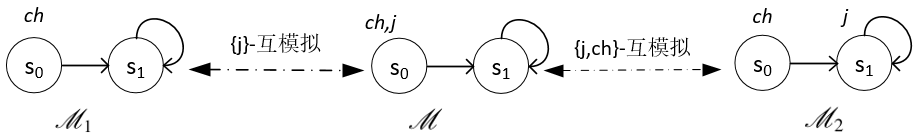
\includegraphics[width=12cm]{figures/chapter06/partial_order2.png}
		\caption{初始结构间的$\leq_{\Hm}$关系。}\label{fig:partialo}
		
		% $s_0$ is labeled by $\{ch, j\}$, $t_0$ is labeled by $\{j\}$, and $s_1$, $s_2$, and $t_1$ are labeled by $\emptyset$.}\label{fig:bisim}
	\end{figure}
\end{example}

给定有限初始结构集$M$和有限初始结构$\Hm$,用$Min(M,$ $\leq_{\Hm})$表示$M$ 中关于偏序关系$\leq_{\Hm}$的极小有限初始结构集。则$\leq_{\Hm}$与知识更新操作$\diamond_{\CTL}$有如下关系。

\begin{theorem}\label{thm:minU}
	给定$\mu$-句子$\Gamma$和$\varphi$,则:
	\[\Mod(\Gamma \diamond_{\CTL} \varphi) = \bigcup_{\Hm\in \Mod(\Gamma)} Min(\Mod(\varphi), \leq_{\Hm}).
	\]
\end{theorem}
\begin{proof}
	$\Hm'\in \Mod(\Gamma \diamond_{\CTL} \varphi)$\\
	$\LRto$ 存在$\Hm \models \Gamma$和极小子集$V_{min} \subseteq \Ha$,使得$\Hm' \in \Mod(\Muforget({\cal F}_{\Ha}(\Hm)$, $V_{min}) \wedge \varphi)$\\
	$\LRto$ 存在$\Hm \models \Gamma$和$V_{min}\subseteq \Ha$,使得$\Hm \lrto_{V_{min}} \Hm'$和$\Hm' \models \varphi$,且$V_{min}$是使得$\Muforget({\cal F}_{\Ha}(\Hm)$, $V_{min}) \wedge \varphi$可满足的$\Ha$ 极小子集\\
	$\LRto$ 存在$\Hm \models \Gamma$,使得对任意$\Hm''\models \varphi$,$\Hm' \leq_{\Hm} \Hm''$\\
	$\LRto$ $\Hm' \in Min(\Mod(\varphi), \leq_{\Hm})$。
\end{proof}


从定理\ref{thm:minU}可以看出,通过遗忘定义的知识更新操作与通过有限初始结构间的偏序关系定义的知识更新一致,且通过遗忘定义的知识更新操作满足Katsuno和Mendelzon提出的八条基本条件。

\begin{theorem}\label{thm:U1toU8}
	知识更新操作$\diamond_{\CTL}$满足Katsuno和Mendelzon提出的基本条件(U1)-(U8)。
\end{theorem}
\begin{proof}
	(U1). 由定理~\ref{thm:minU}可知,$\Mod(\Gamma \diamond_{\mu} \varphi) \subseteq \Mod(\varphi)$,因此$\Gamma \diamond_{\mu} \varphi \models \varphi$。
	
	(U2). $\Hm'\in \Mod(\Gamma \diamond_{\mu} \varphi)$\\
	$\LRto$ 存在$\Hm \models \Gamma$,使得对任意$\Hm'' \models \varphi$ 和$V \subseteq \Ha$,$\Hm'' \lrto_{V} \Hm$ 蕴涵$\Hm' \lrto_{V} \Hm$\\
	$\LRto$ 存在$\Hm \models \Gamma$和$V_{min} = \emptyset$,使得$\Hm' \lrto_{V_{min}} \Hm$ \hfill ($\Gamma \models \varphi$)\\
	$\LRto$ $\Hm'\models \Gamma$。
	
	
	容易证明$\diamond_{\mu}$满足(U3)和(U4)。
	%We now prove (U5).
	
	(U5). $\Hm'\models (\Gamma \diamond_{\mu} \varphi) \wedge \psi$\\
	$\Rto$  存在$\Hm \models \Gamma$,使得对任意$\Hm'' \models \varphi \wedge \psi$ 和$V \subseteq \Ha$,$\Hm'' \lrto_{V} \Hm$蕴涵$\Hm' \lrto_{V} \Hm$\\
	$\Rto$ 存在$\Hm \models \Gamma$和$V_{min} \subseteq \Ha$,使得$\Hm' \lrto_{V_{min}} \Hm$和$\Hm' \models \varphi \wedge \psi$,其中$V_{min}$是使得$\Hm' \lrto_{V_{min}} \Hm$的$\Ha$的极小子集\\
	% 且对任意的$\Hm''\models \psi$ 若$\Hm''\lrto_V \Hm$则$\Hm' \lrto_{V} \Hm$且$V_{min} \subseteq V$ \\
	$\Rto$ $\Hm' \models \Gamma \diamond_{\mu} (\varphi \wedge \psi)$。
	
	
	
	(U6). $\Hm'\models \Gamma \diamond_{\CTL} \varphi$\\
	$\LRto$ 存在$\Hm \models \Gamma$,使得对任意$\Hm'' \models \varphi$ 和$V \subseteq \Ha$,$\Hm'' \lrto_{V} \Hm$ 蕴涵$\Hm' \lrto_{V} \Hm$\\
	$\LRto$ 存在$\Hm \models \Gamma$和$V_{min} \subseteq \Ha$,使得$\Hm' \lrto_{V_{min}} \Hm$,其中$V_{min}$是使得$\Muforget({\cal F}_{\Ha}(\Hm_1), V_{min}) \wedge \varphi$ 和 $\Muforget({\cal F}_{\Ha}(\Hm_1), V_{min}) \wedge \psi$是一致的 \hfill ($\Gamma \diamond_{\CTL} \varphi \models \psi$, $\Gamma \diamond_{\CTL} \psi \models \varphi$) \\ % \qquad \qquad \textcolor[RGB]{0,134,139}{$\%$({\em Otherwise, suppose that $V\subset V_{min}$ s.t. $\Muforget({\cal F}_{\Ha}(\Hm_1), V) \wedge \psi$ is consistent as well. Then, $\Muforget({\cal F}_{\Ha}(\Hm_1), V)$ $\wedge \varphi$ should also be consistent by $\Gamma \diamond_{\CTL} \varphi \models \psi$, which contradicts to the fact that $V_{min}$ is the minimal set of atoms s.t. $\Muforget({\cal F}_{\Ha}(\Hm_1), V_{min}) \wedge \varphi$ is consistent.})} \\
	$\LRto$ 存在$\Hm \models \Gamma$,使得对任意$\Hm'' \models \psi$ 和$V \subseteq \Ha$,$\Hm'' \lrto_{V} \Hm$ 蕴涵$\Hm' \lrto_{V} \Hm$\\
	$\LRto$ $\Hm' \models \Gamma \diamond_{\CTL} \psi$。
	
	
	
	(U7). $\Hm' \models (\Gamma \diamond_{\CTL} \varphi) \wedge (\Gamma \diamond_{\CTL} \psi)$,且设$\Hm$是$\Gamma$的唯一模型\\
	$\Rto$ 存在两个极小子集$V_1, V_2 \subseteq \Ha$,使得$\Hm \lrto_{V_1} \Hm'$ 和$\Hm \lrto_{V_2} \Hm'$\\
	$\Rto$ 存在两个极小子集$V_1, V_2 \subseteq \Ha$,使得$\Hm' \models \Muforget({\cal F}_{\Ha}(\Hm), V_1) \wedge \varphi$ 和 $\Hm' \models \Muforget({\cal F}_{\Ha}(\Hm),$ $V_2) \wedge \psi$是一致的\\
	%$\Rto$ $\Hm' \lrto_{V_1 \cap V_2} \Hm$\\
	$\Rto$ $\Hm' \models \Muforget({\cal F}_{\Ha}(\Hm), V_1 \cap V_2)$,$\Hm' \lrto_{V_1 \cap V_2} \Hm$,$V_1 = V_2$\\
	$\Rto$  $V_1$是使得$\Muforget({\cal F}_{\Ha}(\Hm), V_1) \wedge (\varphi \vee \psi)$可满足的极小子集\\ %\qquad  \textcolor[RGB]{0,134,139}{$\%$({\em Otherwise, suppose that $V_3\subset V_1$ s.t. $\Muforget({\cal F}_{\Ha}(\Hm),$ $V_3) \wedge (\varphi \vee \psi)$ is satisfiable. Then $\Muforget({\cal F}_{\Ha}(\Hm),$ $V_3) \wedge \varphi$ or $\Muforget({\cal F}_{\Ha}(\Hm),$ $V_3) \wedge \psi$ is satisfiable. Without loss of generality, suppose that $\Muforget({\cal F}_{\Ha}(\Hm), V_3) \wedge \varphi$ is satisfiable, $V_1$ is not the minimal set, a contradiction.})}\\
	$\Rto$ $\Hm' \models \Gamma \diamond_{\CTL} (\varphi \vee \psi)$。
	
	
	
	(U8). $\Hm \models (\Gamma_1 \vee \Gamma_2) \diamond_{\CTL} \varphi$ \\
	$\LRto$ 存在$\Hm_1 \models \Gamma_1$ (或$\Hm_1 \models \Gamma_2$) 和一个极小子集$V_{min}$,使得$\Hm \lrto_{V_{min}} \Hm_1$\\
	$\LRto$ $\Hm \models (\Gamma_1 \diamond_{\CTL} \varphi) \vee (\Gamma_2 \diamond_{\CTL} \varphi)$。
\end{proof}


\begin{example}
	令$\Ha=\{ch, j\}$、$\varphi = \nu X. j \wedge ch \wedge \EXIST \NEXT \EXIST \NEXT X$、 $\psi= \nu X. \neg j \wedge ch \wedge \EXIST \NEXT \EXIST \NEXT X$且Kripke结构的状态空间为 $\{s_0,s_1\}$,则用$\psi$更新$\varphi$ 计算如下:
	\begin{align*}
		\Mod(\varphi) = & \{((1), r=s_0, L(s_0)=\{ch,j\}, L(s_1)=\{ch,j\}), \\
		& ((2),  r=s_1, L(s_1)=\{ch,j\}, L(s_0)=\{ch,j\}),\\
		& ((3),  r=s_0, L(s_0)=\{ch,j\}, L(s_1)={\cal C}), \\
		& ((4),  r=s_1, L(s_1)=\{ch,j\}, L(s_0)={\cal C}), \\
		& ((5),  r=s_0, L(s_0)=\{ch,j\}, L(s_1)={\cal C}), \\
		& ((6),  r=s_1, L(s_1)=\{ch,j\}, L(s_0)={\cal C}), \dots\}\\
		\Mod(\psi) = & \{((1), r=s_0, L(s_0)=\{ch\}, L(s_1)=\{ch\}),\\
		& ((2), r=s_1, L(s_1)=\{ch\}, L(s_0)=\{ch\}),\\
		& ((3), r=s_0, L(s_0)=\{ch\}, L(s_1)={\cal C}),\\
		& ((4), r=s_1, L(s_1)=\{ch\}, L(s_0)={\cal C}), \\
		& ((5), r=s_0, L(s_0)=\{ch\}, L(s_1)={\cal C}),\\
		& ((6), r=s_1, L(s_1)=\{ch\}, L(s_0)={\cal C}), \dots\}
	\end{align*}
	其中,四元组$((i), r= s_k, L(s_0)=V_1, L(s_1)=V_1)$表示Kripke结构$(S,r,R,L)$,其中$S=\{s_0, s_1\}$、$r=s_k$ ($r\in \{0,1\}$)、转换关系如图~\ref{fig:knoup}中的(i) ($i \in \{1,2,3,4,5,6\}$\footnote{这里只列出部分转换关系,其余转换关系可以容易地枚举出来。})、$s_0$ 和$s_1$分别被 $V_1 \subseteq \{ch,j\}$ 和 $V_2\subseteq \{ch,j\}$标记且${\cal C} \in \{\emptyset, \{j\}, \{ch\}, \{j,ch\}\}$。
	
	$\Mod(\varphi \diamond_{\mu} \psi) = \bigcup_{\Hm\in \Mod(\varphi)} Min(\Mod(\psi), \leq_{\Hm})$,根据定义~\ref{def:closer}容易检查$\Mod(\varphi \diamond_{\mu} \psi) = \Mod(\psi)$。直观地说,由于在$\psi$中$j$在偶数状态不再为真、$ch$保持为真且$\psi$和$\varphi$ 都不知道模型偶数状态的信息,因而用$\psi$更新$\varphi$得到的结果为 $\psi$ 自身。
	\begin{figure}[h]%
		\centering
		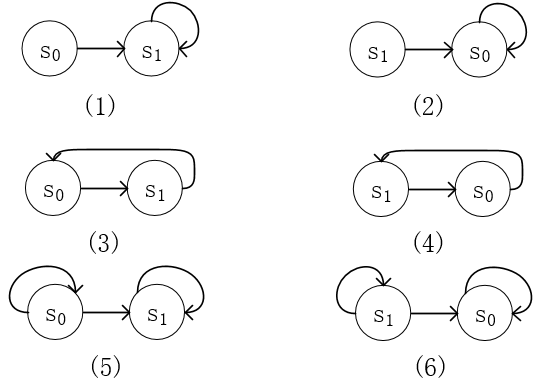
\includegraphics[width=8cm]{knowledge_update.png}
		\caption{状态空间为$\{s_0,s_1\}$的六个Kripke结构示意图}\label{fig:knoup}
		
		% $s_0$ is labeled by $\{ch, j\}$, $t_0$ is labeled by $\{j\}$, and $s_1$, $s_2$, and $t_1$ are labeled by $\emptyset$.}\label{fig:bisim}
	\end{figure}
\end{example}


\section{本章小结}\label{sec:chapter04-conclusion}

本章讨论了如何使用遗忘计算最强必要条件(最弱充分条件)和定义知识更新。
为此,本章第一节首先提出了一种有界$V$-互模拟概念,并证明了该有界$V$-互模拟与$V$-互模拟在有限结构下是等价的。定义了给定深度的计算树在给定原子命题集上的特征公式,由此定义了有限初始结构的特征公式。结论表明初始结构能够满足给定的特征公式当且仅当该初始结构与特征公式对应的初始结构在给定原子命题集上互模拟。
此外,本章首先给出了SNC(WSC)的定义,表明SNC和WSC是一对对偶概念,因而只要知道其一就能知道另一个。其次,结论表明任意公式的SNC(WSC)可以转换成原子命题的SNC (WSC)来计算,并给出使用遗忘计算原子命题在给定条件下的SNC(WSC)的方法,从而根据初始结构的特征公式计算出反应式系统的SNC(WSC)。
最后,分别给出使用遗忘和偏序关系的方法定义知识更新,并证明了这两种定义等价且满足Katsuno等人提出的八条准则。

